% Options for packages loaded elsewhere
\PassOptionsToPackage{unicode}{hyperref}
\PassOptionsToPackage{hyphens}{url}
\PassOptionsToPackage{dvipsnames,svgnames,x11names}{xcolor}
%
\documentclass[
]{article}
\usepackage{amsmath,amssymb}
\usepackage{iftex}
\ifPDFTeX
  \usepackage[T1]{fontenc}
  \usepackage[utf8]{inputenc}
  \usepackage{textcomp} % provide euro and other symbols
\else % if luatex or xetex
  \usepackage{unicode-math} % this also loads fontspec
  \defaultfontfeatures{Scale=MatchLowercase}
  \defaultfontfeatures[\rmfamily]{Ligatures=TeX,Scale=1}
\fi
\usepackage{lmodern}
\ifPDFTeX\else
  % xetex/luatex font selection
\fi
% Use upquote if available, for straight quotes in verbatim environments
\IfFileExists{upquote.sty}{\usepackage{upquote}}{}
\IfFileExists{microtype.sty}{% use microtype if available
  \usepackage[]{microtype}
  \UseMicrotypeSet[protrusion]{basicmath} % disable protrusion for tt fonts
}{}
\makeatletter
\@ifundefined{KOMAClassName}{% if non-KOMA class
  \IfFileExists{parskip.sty}{%
    \usepackage{parskip}
  }{% else
    \setlength{\parindent}{0pt}
    \setlength{\parskip}{6pt plus 2pt minus 1pt}}
}{% if KOMA class
  \KOMAoptions{parskip=half}}
\makeatother
\usepackage{xcolor}
\usepackage[margin=1in]{geometry}
\usepackage{longtable,booktabs,array}
\usepackage{calc} % for calculating minipage widths
% Correct order of tables after \paragraph or \subparagraph
\usepackage{etoolbox}
\makeatletter
\patchcmd\longtable{\par}{\if@noskipsec\mbox{}\fi\par}{}{}
\makeatother
% Allow footnotes in longtable head/foot
\IfFileExists{footnotehyper.sty}{\usepackage{footnotehyper}}{\usepackage{footnote}}
\makesavenoteenv{longtable}
\usepackage{graphicx}
\makeatletter
\def\maxwidth{\ifdim\Gin@nat@width>\linewidth\linewidth\else\Gin@nat@width\fi}
\def\maxheight{\ifdim\Gin@nat@height>\textheight\textheight\else\Gin@nat@height\fi}
\makeatother
% Scale images if necessary, so that they will not overflow the page
% margins by default, and it is still possible to overwrite the defaults
% using explicit options in \includegraphics[width, height, ...]{}
\setkeys{Gin}{width=\maxwidth,height=\maxheight,keepaspectratio}
% Set default figure placement to htbp
\makeatletter
\def\fps@figure{htbp}
\makeatother
\setlength{\emergencystretch}{3em} % prevent overfull lines
\providecommand{\tightlist}{%
  \setlength{\itemsep}{0pt}\setlength{\parskip}{0pt}}
\setcounter{secnumdepth}{-\maxdimen} % remove section numbering
\newlength{\cslhangindent}
\setlength{\cslhangindent}{1.5em}
\newlength{\csllabelwidth}
\setlength{\csllabelwidth}{3em}
\newlength{\cslentryspacingunit} % times entry-spacing
\setlength{\cslentryspacingunit}{\parskip}
\newenvironment{CSLReferences}[2] % #1 hanging-ident, #2 entry spacing
 {% don't indent paragraphs
  \setlength{\parindent}{0pt}
  % turn on hanging indent if param 1 is 1
  \ifodd #1
  \let\oldpar\par
  \def\par{\hangindent=\cslhangindent\oldpar}
  \fi
  % set entry spacing
  \setlength{\parskip}{#2\cslentryspacingunit}
 }%
 {}
\usepackage{calc}
\newcommand{\CSLBlock}[1]{#1\hfill\break}
\newcommand{\CSLLeftMargin}[1]{\parbox[t]{\csllabelwidth}{#1}}
\newcommand{\CSLRightInline}[1]{\parbox[t]{\linewidth - \csllabelwidth}{#1}\break}
\newcommand{\CSLIndent}[1]{\hspace{\cslhangindent}#1}
\usepackage{fancyhdr}
\pagestyle{fancy}
\fancyhf{}
\lfoot[\thepage]{}
\rfoot[]{\thepage}
\fontsize{12}{22}
\selectfont
\usepackage{booktabs}
\usepackage{longtable}
\usepackage{array}
\usepackage{multirow}
\usepackage{wrapfig}
\usepackage{float}
\usepackage{colortbl}
\usepackage{pdflscape}
\usepackage{tabu}
\usepackage{threeparttable}
\usepackage{threeparttablex}
\usepackage[normalem]{ulem}
\usepackage{makecell}
\usepackage{xcolor}
\ifLuaTeX
  \usepackage{selnolig}  % disable illegal ligatures
\fi
\IfFileExists{bookmark.sty}{\usepackage{bookmark}}{\usepackage{hyperref}}
\IfFileExists{xurl.sty}{\usepackage{xurl}}{} % add URL line breaks if available
\urlstyle{same}
\hypersetup{
  colorlinks=true,
  linkcolor={blue},
  filecolor={Maroon},
  citecolor={Blue},
  urlcolor={Blue},
  pdfcreator={LaTeX via pandoc}}

\title{
\includegraphics[width=10cm,height=\textheight]{IEO-logo2.png}}
\author{}
\date{\vspace{-2.5em}}

\begin{document}
\maketitle


\pagenumbering{gobble}

%\begin{titlepage}
\begin{flushleft}
\Large{\textbf{Entregble 2. Reporte (Preliminar) Stock Assessment}}\\
\vspace*{2\baselineskip}
\LARGE{\textbf{Implementación metodológica de evaluación de stock en coquina \textit{Donax trunculus} en SS3 en el Golfo de Cádiz, España}}\\
\vspace*{5\baselineskip}
\Large{Grupo de Trabajo FEMP 04}\\
\vspace*{1\baselineskip}
\Large{Instituto Español de Oceanografía, Cádiz }\\
\vspace*{4\baselineskip}
\end{flushleft}
\begin{flushright}
\large{\textit{Mauricio Mardones}}\\
\large{\textit{Marina Delgado}}\\
\vspace*{1\baselineskip}
\normalsize{\textbf{Fecha}}\\
Abril, 2024
\end{flushright}

% \end{titlepage}


\hypersetup{linkcolor = black}
\newpage
\pagenumbering{roman}
%\tableofcontents
%\addcontentsline{toc}{section}{\contentsname}

\newpage



\pagenumbering{arabic}
\hypersetup{linkcolor = blue}

{
\hypersetup{linkcolor=}
\setcounter{tocdepth}{3}
\tableofcontents
}
\pagebreak

\hypertarget{contexto}{%
\section{1. CONTEXTO}\label{contexto}}

El objetivo de este documento es la implementación metodológica de la evaluación de stock de coquina \emph{Donax trunculus} mediante un modelo integrado con datos en talla y dinamica en edad implemetnado en Stock Synthesis (SS3) (v.3.30.21) (\protect\hyperlink{ref-Methot2023}{Richard D. Methot et al., 2023}; \protect\hyperlink{ref-Methot2013}{Richard D. Methot \& Wetzel, 2013}) para la zona del Golfo de Cádiz, España. Este trabajo está en el marco de la asesoría científica que lleva a cabo el Instituto Español de Oceanografía (IEO) realizado por el grupo de investigadores asociados al proyecto FEMP 04.

A su vez, se destaca la utilidad de los programas de monitoreo de la población y la pesquería que se ejecutan desde el año 2013 por parte del IEO Cádiz, y con el cual se ha levantado informacion biológica, pesquera y ambiental que ha sido vital para estea implementación metodológica, consitituyendo así el primer ejercicio de evaluación de stock de coquina.

\hypertarget{metodologuxeda}{%
\section{2. METODOLOGÍA}\label{metodologuxeda}}

El flujo de trabajo asociado a la modelación de stock, tanto componentes como fuentes de datos está representado de forma genérica en el siguiente diagrama de flujo (Figura \ref{fig:esq});

\begin{figure}

{\centering \includegraphics[width=1\linewidth]{FIg/Diagrama_Modelo} 

}

\caption{\label{fig:esq}Esquema de modelación de coquina}\label{fig:esq}
\end{figure}

\pagebreak

\hypertarget{datos-utilizados}{%
\subsection{2.1. Datos utilizados}\label{datos-utilizados}}

Los datos analizados que formaron parte de los inputs del modelo fueron clasificados de acuerdo a su origen. A saber;

\begin{enumerate}
\def\labelenumi{\alph{enumi}.}
\item
  Desembarque artesanal del período (2004-2024), provenientes de las estadisticas oficiales de \href{https://www.juntadeandalucia.es/agriculturaypesca/idapes/servlet/FrontController}{IDAPES} asociados al sector de marisquería del Parque Doñana y cercanías. Cabe señalar que en esta pesquería aun no se realizan procesos de corrección de desembarques y que serán propuestos como escenarios de modelación.
\item
  Información de los programas de monitoreo poblacional y comercial que lleva a cabo el IEO desee el año 2013. En este monitoreo se recopila información biológica, pesquera y ambiental.
\end{enumerate}

c . Información relativa a los parámetros de historia de vida de la coquina a nivel europeo y local. Esta información está contenida en artículos científicos y reportes que fueron compilados con el fin de parametrizar los modelos de evaluación.

Toda esta información, codigos fuente, bases de datos y Analisis Exploratorio de Datos puede ser encontrado en el siguiente enlace: \href{https://mauromardones.github.io/EDA_Donux_trunculus_2023/}{Data coquina}. La cobertura temporal de las fuentes de datos varia de acuerdo a la disponibilidad asociada al programa y fuente (Figura \ref{fig:data});

\begin{figure}[H]

{\centering \includegraphics[width=0.8\linewidth]{s1/plots/data_plot} 

}

\caption{\label{fig:data}Cobertura temporal de las distintas fuentes de datos usadas en el modelo implementado en SS3 para coquina}\label{fig:data}
\end{figure}

\hypertarget{modelo-de-la-dinuxe1mica-poblacional}{%
\subsection{2.2. Modelo de la dinámica poblacional}\label{modelo-de-la-dinuxe1mica-poblacional}}

El modelo de dinámica poblacional de la coquina, corresponde a un enfoque de evaluación del tipo estadístico con estructura de edad, donde la dinámica progresa avanzando en el tiempo t, y las capturas son causantes de la mortalidad por pesca F, la mortalidad natural es constante \texttt{M\ =\ 0.99} (Tabla \ref{Tab1}). La relación entre la población y las capturas responde a la base de la ecuación de Baranov, y se consideran para el modelo y estimaciones el rango de edad entre 1 a 5+ (años). Sin embargo, las estimaciones del modelo tienen su origen en la edad cero sobre la base de una condición inicial estado estable. La dinámica esta modelada por un reclutamiento tipo Beverton y Holt.

De manera sencilla, un modelo de evaluación reproduce la dinámica poblacional de coquina a lo largo del tiempo. Este modelo incorpora parámetros biológicos clave como tasas de crecimiento, tasas de mortalidad, reclutamiento y biomasa desovante. Normalmente, el modelo se formula utilizando ecuaciones matemáticas que describen cómo estos parámetros interactúan para determinar la abundancia y distribución de coquina en el área de estudio. La ecuación de estado de creciiento poblacional de coquina puede representarse como:

\[
N_t = N_{t-1} \cdot e^{(r - M)} + R
\]

Donde:
- \(N_t\) es abundancia de coquina en el tiempo \(t\).
- \(N_{t-1}\) abundancia de krill en pasos de tiempo previos.
- \(r\) es la tasa de crecimiento poblacional intrinseca.
- \(M\) es la tasa de mortalidad natural.
- \(R\) es el reclutamiento de nuevos individuos al stock.

\hypertarget{plataforma-de-evaluacion-de-stock}{%
\subsection{2.3. Plataforma de Evaluacion de Stock}\label{plataforma-de-evaluacion-de-stock}}

La ecuación descrita en el punto \texttt{2.2} describe la dinámica básica de la población de coquina, con la abundancia cambiando con el tiempo debido al crecimiento, la mortalidad y el reclutamiento. Junto a esta ecuación, otros submodelos asociados como crecimiento individual, selectividad, madurez, captura a la edad entre otros estan configurados en SS3. Este plataforma de evaluación de stock está diseñada como un modelo estructurado con dinámica en edad y datos en talla, en la clase de modelo denominado \emph{Modelo de análisis integrado}. SS3 tiene un sub-modelo poblacional de stock que simula crecimiento, madurez, fecundidad, reclutamiento, movimiento, y procesos de mortalidad, y sub-modelos de observation y valores esperados para diferentes tipos de datos. El modelo es codificado en C++ con parámetros de estimación activados por diferenciación automática (ADMB) (\protect\hyperlink{ref-Methot2013}{Richard D. Methot \& Wetzel, 2013}). El análisis de resultados y salidas emplea herramientas de R e interfase gráfica de la librería \texttt{r4ss} (\url{https://github.com/r4ss/r4ss}) (\protect\hyperlink{ref-Taylor2019}{Taylor, 2019}) y \texttt{ss3diags} (\protect\hyperlink{ref-Henning2023}{Winker et al., 2023}).

Las rutinas y datos de este proceso metodologico de evaluaciónpueden ser encontrados en el repositorio de \href{https://github.com/MauroMardones/SA_Donax_trunculus.}{SA\_Donax\_trunculus}

\hypertarget{modelo-base-condicionamiento}{%
\subsection{2.4. Modelo Base (Condicionamiento)}\label{modelo-base-condicionamiento}}

La estimación de la biomasa desovante se realizó a inicios de año, mientras que el reclutamiento se consideró como un evento doble que ocurre hacia junio y fines de año. En el proceso de estimación del reclutamiento, se incorporó una relación stock-recluta difusa (steepness 0.7), y las variaciones en el reclutamiento se modelaron como desviaciones del reclutamiento virginal \texttt{R0}, asumiendo 2004 como año inicial (Tabla \ref{Tab1}).

La mortalidad por pesca se estimó como el promedio simple de la \texttt{F} de las clases de edad 1 y 2, lo que en el modelo corresponde a la opción 5 del método \texttt{F\ híbrido} recomendado en SS3 (\protect\hyperlink{ref-Methot2013}{Richard D. Methot \& Wetzel, 2013}). Se asume que la densidad es un proxi de las biomasas estimadas (\protect\hyperlink{ref-Caddy2004}{Caddy, 2004}) obtenida desde los muestreos poblacionales y que son proporcionales a la biomasa vulnerable de la población, con la capturabilidad (\texttt{q}) estimada en el modelo. Los parámetros \texttt{q} fueron estimados a patir de parámetros iniciales especificados en la Tabla \ref{Tab1} para los datos del monitoreo poblacional , así como del comercial. Todos los patrones de selectividad, que relacionan las composiciones de tallas observadas de la flota comercial y poblacional con la dinámica, fueron estimados mediante una función logística. Los parámetros \texttt{p1} (talla en la inflexión de la curva) y \texttt{p2} (selección al 95\%) son estimados por el modelo a partir de los valores iniciales especificados en la Tabla \ref{Tab1}.

\begin{table}[ht!]
\centering\centering
\caption{\label{tab:unnamed-chunk-8}\label{Tab1}Parámetros de entrada al modelo inicial SS3 de coquina (S1). Cada línea de parámetro contiene un valor mínimo (LO), máximo (HI) e inicial (INIT). Si la fase (PHASE) para el parámetro es negativa, el parámetro es fijo de entrada}
\centering
\fontsize{9}{11}\selectfont
\begin{tabular}[t]{lcccc}
\toprule
  & LO & HI & INIT & PHASE\\
\midrule
\addlinespace[0.3em]
\multicolumn{5}{l}{\textbf{Mortalidad natural}}\\
\hspace{1em}\cellcolor{gray!10}{Nat M} & \cellcolor{gray!10}{0.05} & \cellcolor{gray!10}{2.00} & \cellcolor{gray!10}{0.9900} & \cellcolor{gray!10}{-3}\\
\addlinespace[0.3em]
\multicolumn{5}{l}{\textbf{Crecimiento}}\\
\hspace{1em}Lmin & 1.00 & 3.50 & 2.3000 & 5\\
\hspace{1em}\cellcolor{gray!10}{Lmax} & \cellcolor{gray!10}{2.00} & \cellcolor{gray!10}{8.00} & \cellcolor{gray!10}{4.9000} & \cellcolor{gray!10}{-3}\\
\hspace{1em}VonBert K & 0.08 & 0.80 & 0.4800 & -1\\
\hspace{1em}\cellcolor{gray!10}{CV young} & \cellcolor{gray!10}{0.05} & \cellcolor{gray!10}{0.50} & \cellcolor{gray!10}{0.3000} & \cellcolor{gray!10}{-3}\\
\hspace{1em}CV old & 0.05 & 0.25 & 0.1000 & -3\\
\addlinespace[0.3em]
\multicolumn{5}{l}{\textbf{Relación longitud-peso}}\\
\hspace{1em}\cellcolor{gray!10}{Wt a} & \cellcolor{gray!10}{0.00} & \cellcolor{gray!10}{3.00} & \cellcolor{gray!10}{0.0003} & \cellcolor{gray!10}{-5}\\
\hspace{1em}Wt b & 0.00 & 6.00 & 2.6800 & -5\\
\addlinespace[0.3em]
\multicolumn{5}{l}{\textbf{Ojiva de madurez}}\\
\hspace{1em}\cellcolor{gray!10}{L50\%} & \cellcolor{gray!10}{0.00} & \cellcolor{gray!10}{3.00} & \cellcolor{gray!10}{1.0400} & \cellcolor{gray!10}{-5}\\
\hspace{1em}Mat slope & -3.00 & 3.00 & -1.7000 & -3\\
\addlinespace[0.3em]
\multicolumn{5}{l}{\textbf{Relación stock-recluta}}\\
\hspace{1em}\cellcolor{gray!10}{SR\_LN(R0)} & \cellcolor{gray!10}{3.00} & \cellcolor{gray!10}{50.00} & \cellcolor{gray!10}{25.0000} & \cellcolor{gray!10}{1}\\
\hspace{1em}SR\_BH\_steep & 0.20 & 1.00 & 0.7500 & 4\\
\hspace{1em}\cellcolor{gray!10}{SR\_sigmaR} & \cellcolor{gray!10}{0.00} & \cellcolor{gray!10}{1.00} & \cellcolor{gray!10}{0.2000} & \cellcolor{gray!10}{-4}\\
\hspace{1em}SR\_regime & -5.00 & 5.00 & 0.1000 & -4\\
\hspace{1em}\cellcolor{gray!10}{SR\_autocorr} & \cellcolor{gray!10}{0.00} & \cellcolor{gray!10}{0.00} & \cellcolor{gray!10}{0.0000} & \cellcolor{gray!10}{99}\\
\addlinespace[0.3em]
\multicolumn{5}{l}{\textbf{Capturabilidad}}\\
\hspace{1em}LnQ\_base\_COMERCIAL(1) & -15.00 & 1.50 & -10.0000 & 4\\
\hspace{1em}\cellcolor{gray!10}{LnQ\_base\_POBLACIONAL(2)} & \cellcolor{gray!10}{-15.00} & \cellcolor{gray!10}{1.50} & \cellcolor{gray!10}{-5.0000} & \cellcolor{gray!10}{4}\\
\addlinespace[0.3em]
\multicolumn{5}{l}{\textbf{Selectividad}}\\
\hspace{1em}SizeSel\_P\_1\_COMERCIAL(1) & 0.02 & 4.00 & 0.5000 & 2\\
\hspace{1em}\cellcolor{gray!10}{SizeSel\_P\_2\_COMERCIAL(1)} & \cellcolor{gray!10}{0.01} & \cellcolor{gray!10}{4.00} & \cellcolor{gray!10}{2.5000} & \cellcolor{gray!10}{2}\\
\hspace{1em}SizeSel\_P\_1\_POBLACIONAL(2) & 0.02 & 3.00 & 0.5000 & 2\\
\hspace{1em}\cellcolor{gray!10}{SizeSel\_P\_2\_POBLACIONAL(2)} & \cellcolor{gray!10}{0.01} & \cellcolor{gray!10}{3.00} & \cellcolor{gray!10}{0.5000} & \cellcolor{gray!10}{2}\\
\bottomrule
\end{tabular}
\end{table}

Respecto a los valores y parametros biologicos modelados, los siguientes graficos (Figura \ref{fig:bio}) identifican los estimadores puntuales del recurso

\begin{figure}[H]

{\centering 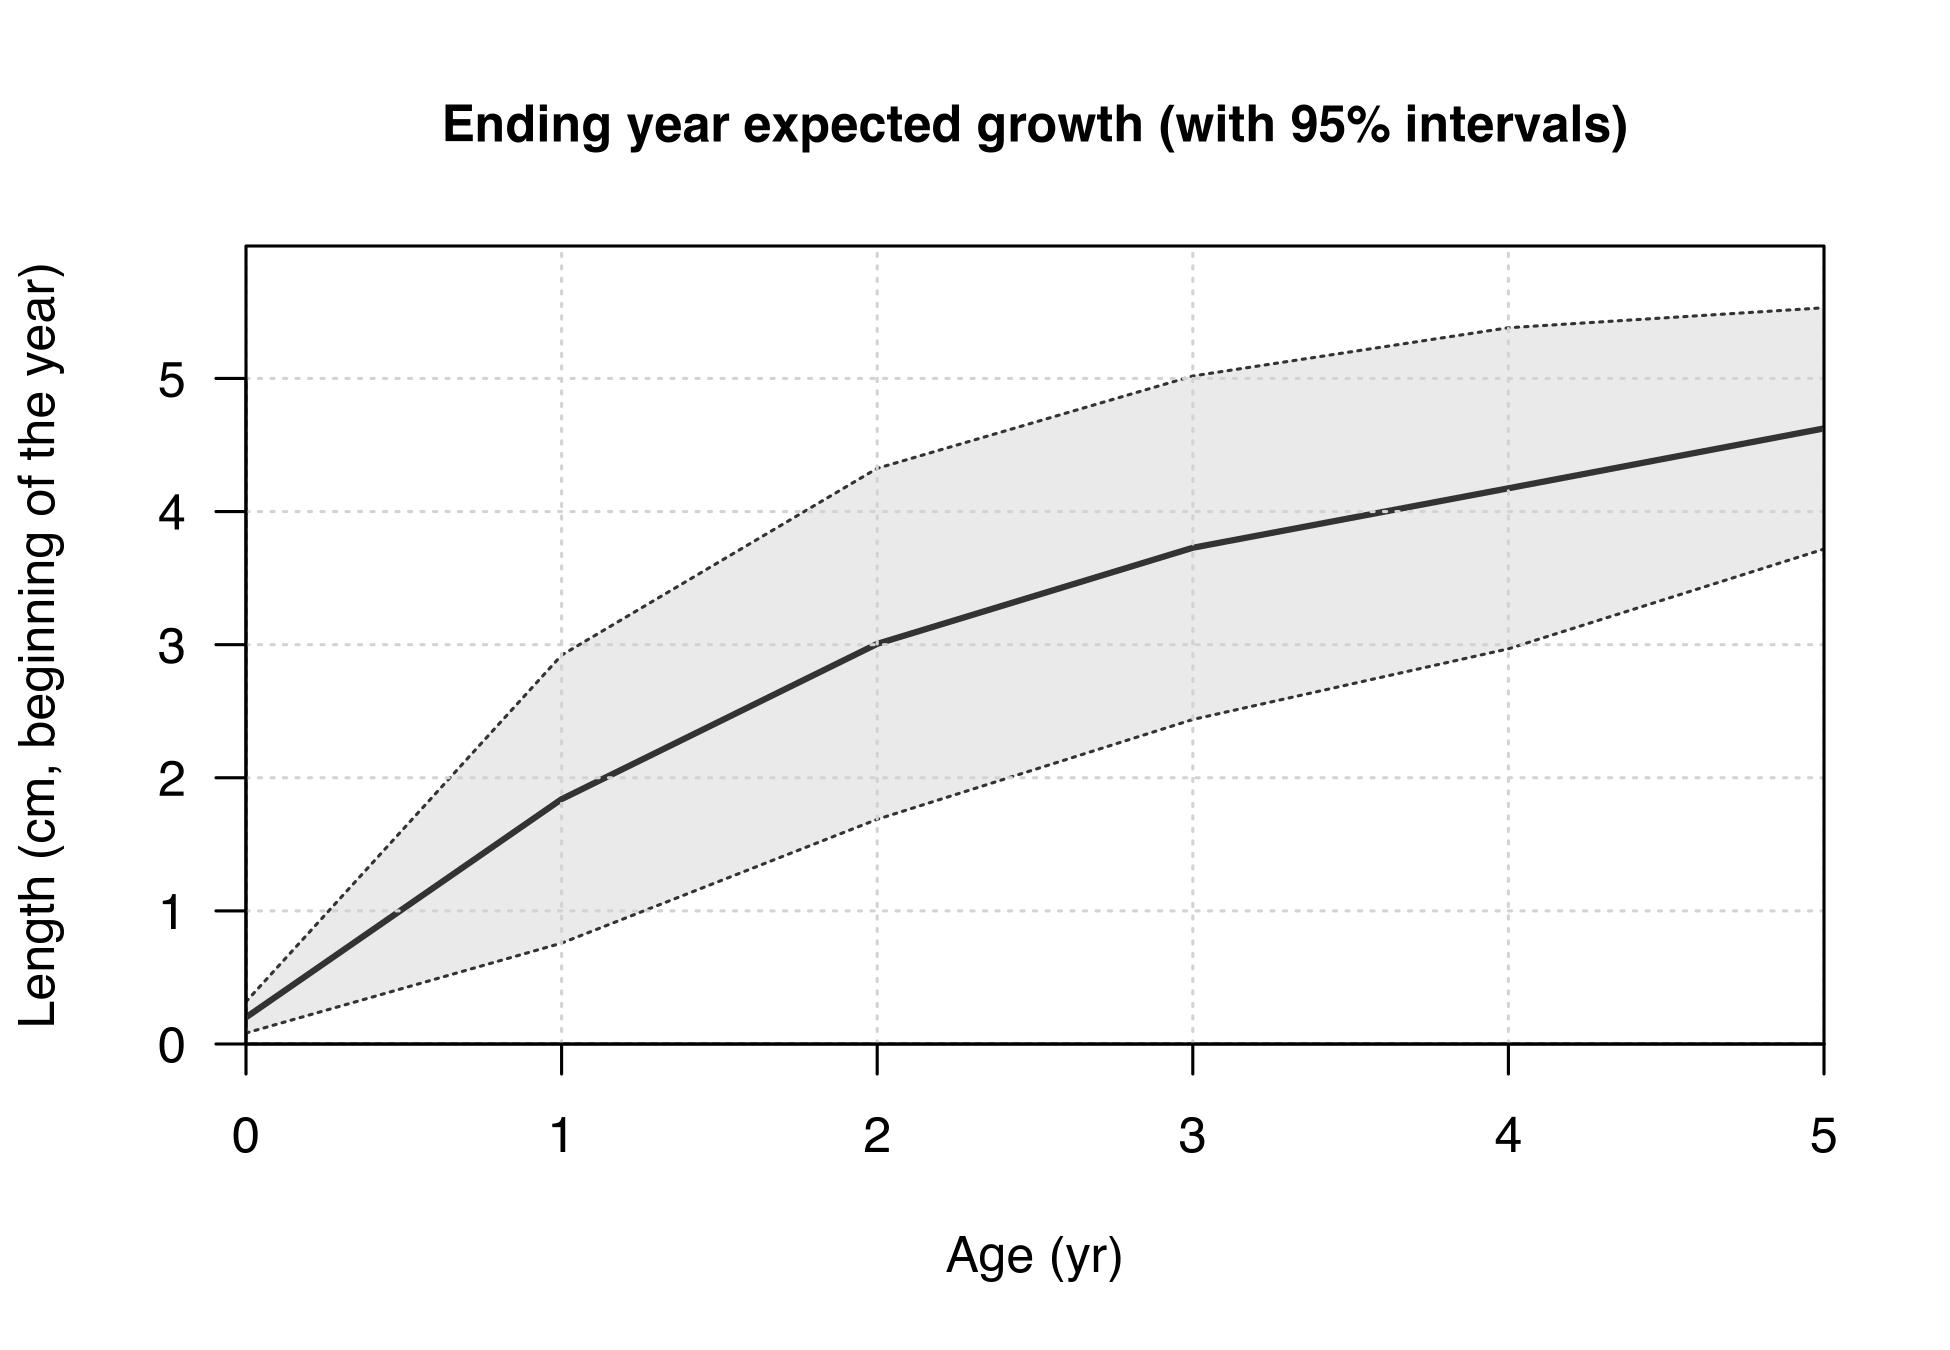
\includegraphics[width=0.8\linewidth]{Dtrunculus_SS3_2024_files/figure-latex/bio-1} 

}

\caption{\label{fig:bio}Función de crecimiento asumida en el modelo. El área sombreada indica una distribución del 95\% de la talla por edad alrededor de la curva de crecimiento estimada y Ojiva de madurez por talla para coquina}\label{fig:bio-1}
\end{figure}
\begin{figure}[H]

{\centering 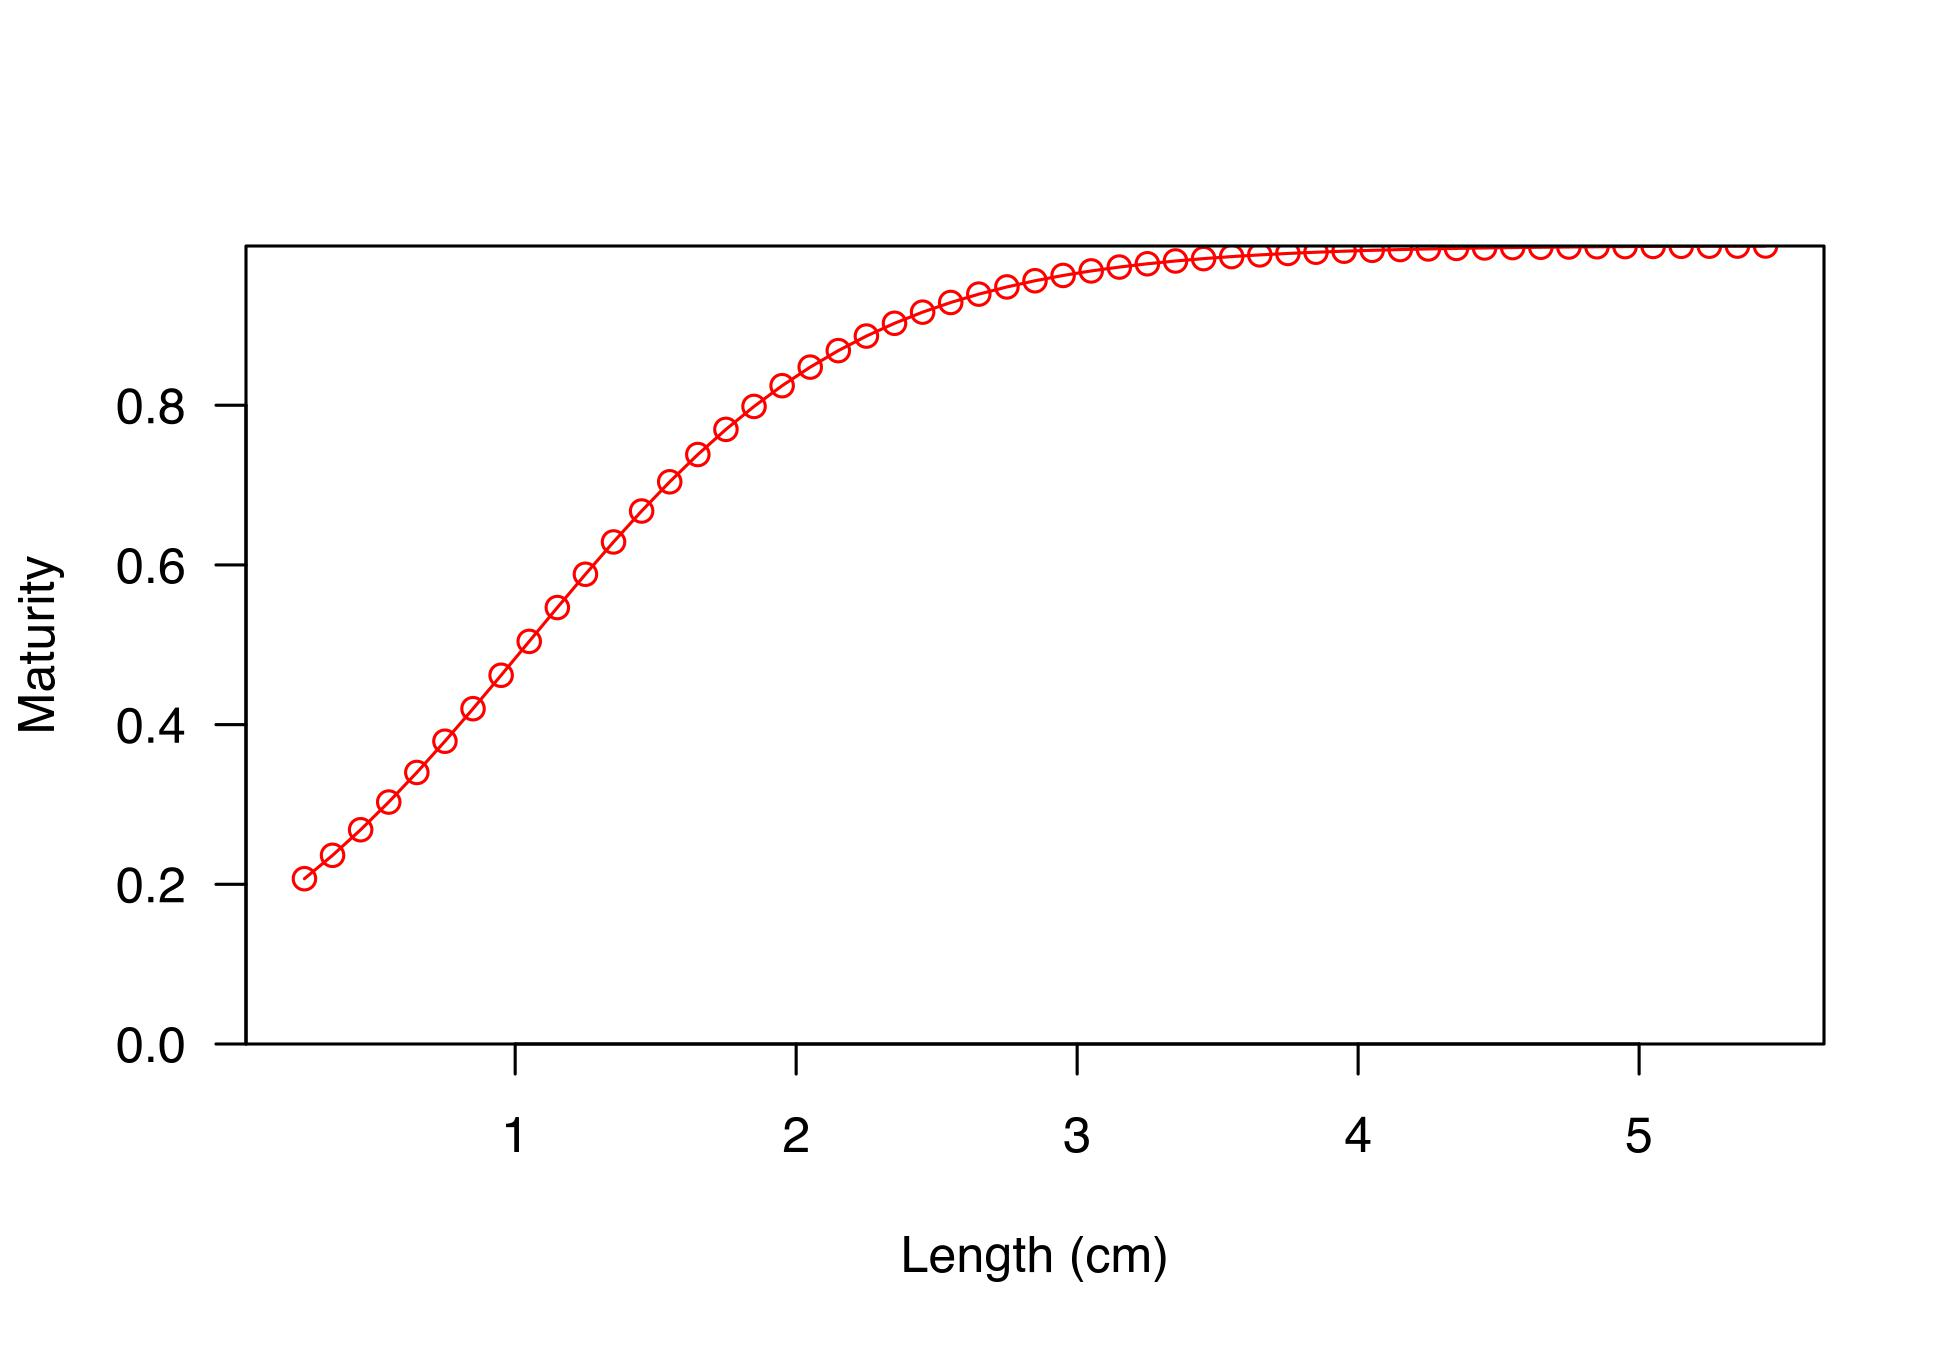
\includegraphics[width=0.8\linewidth]{Dtrunculus_SS3_2024_files/figure-latex/bio-2} 

}

\caption{\label{fig:bio}Función de crecimiento asumida en el modelo. El área sombreada indica una distribución del 95\% de la talla por edad alrededor de la curva de crecimiento estimada y Ojiva de madurez por talla para coquina}\label{fig:bio-2}
\end{figure}

Por otro lado, y al existir dos tipos de muestreos, uno poblacional y otro comercial, se modelan las selectividades por separado como se identifica en la Figura \ref{fig:sel}

\begin{figure}[H]

{\centering 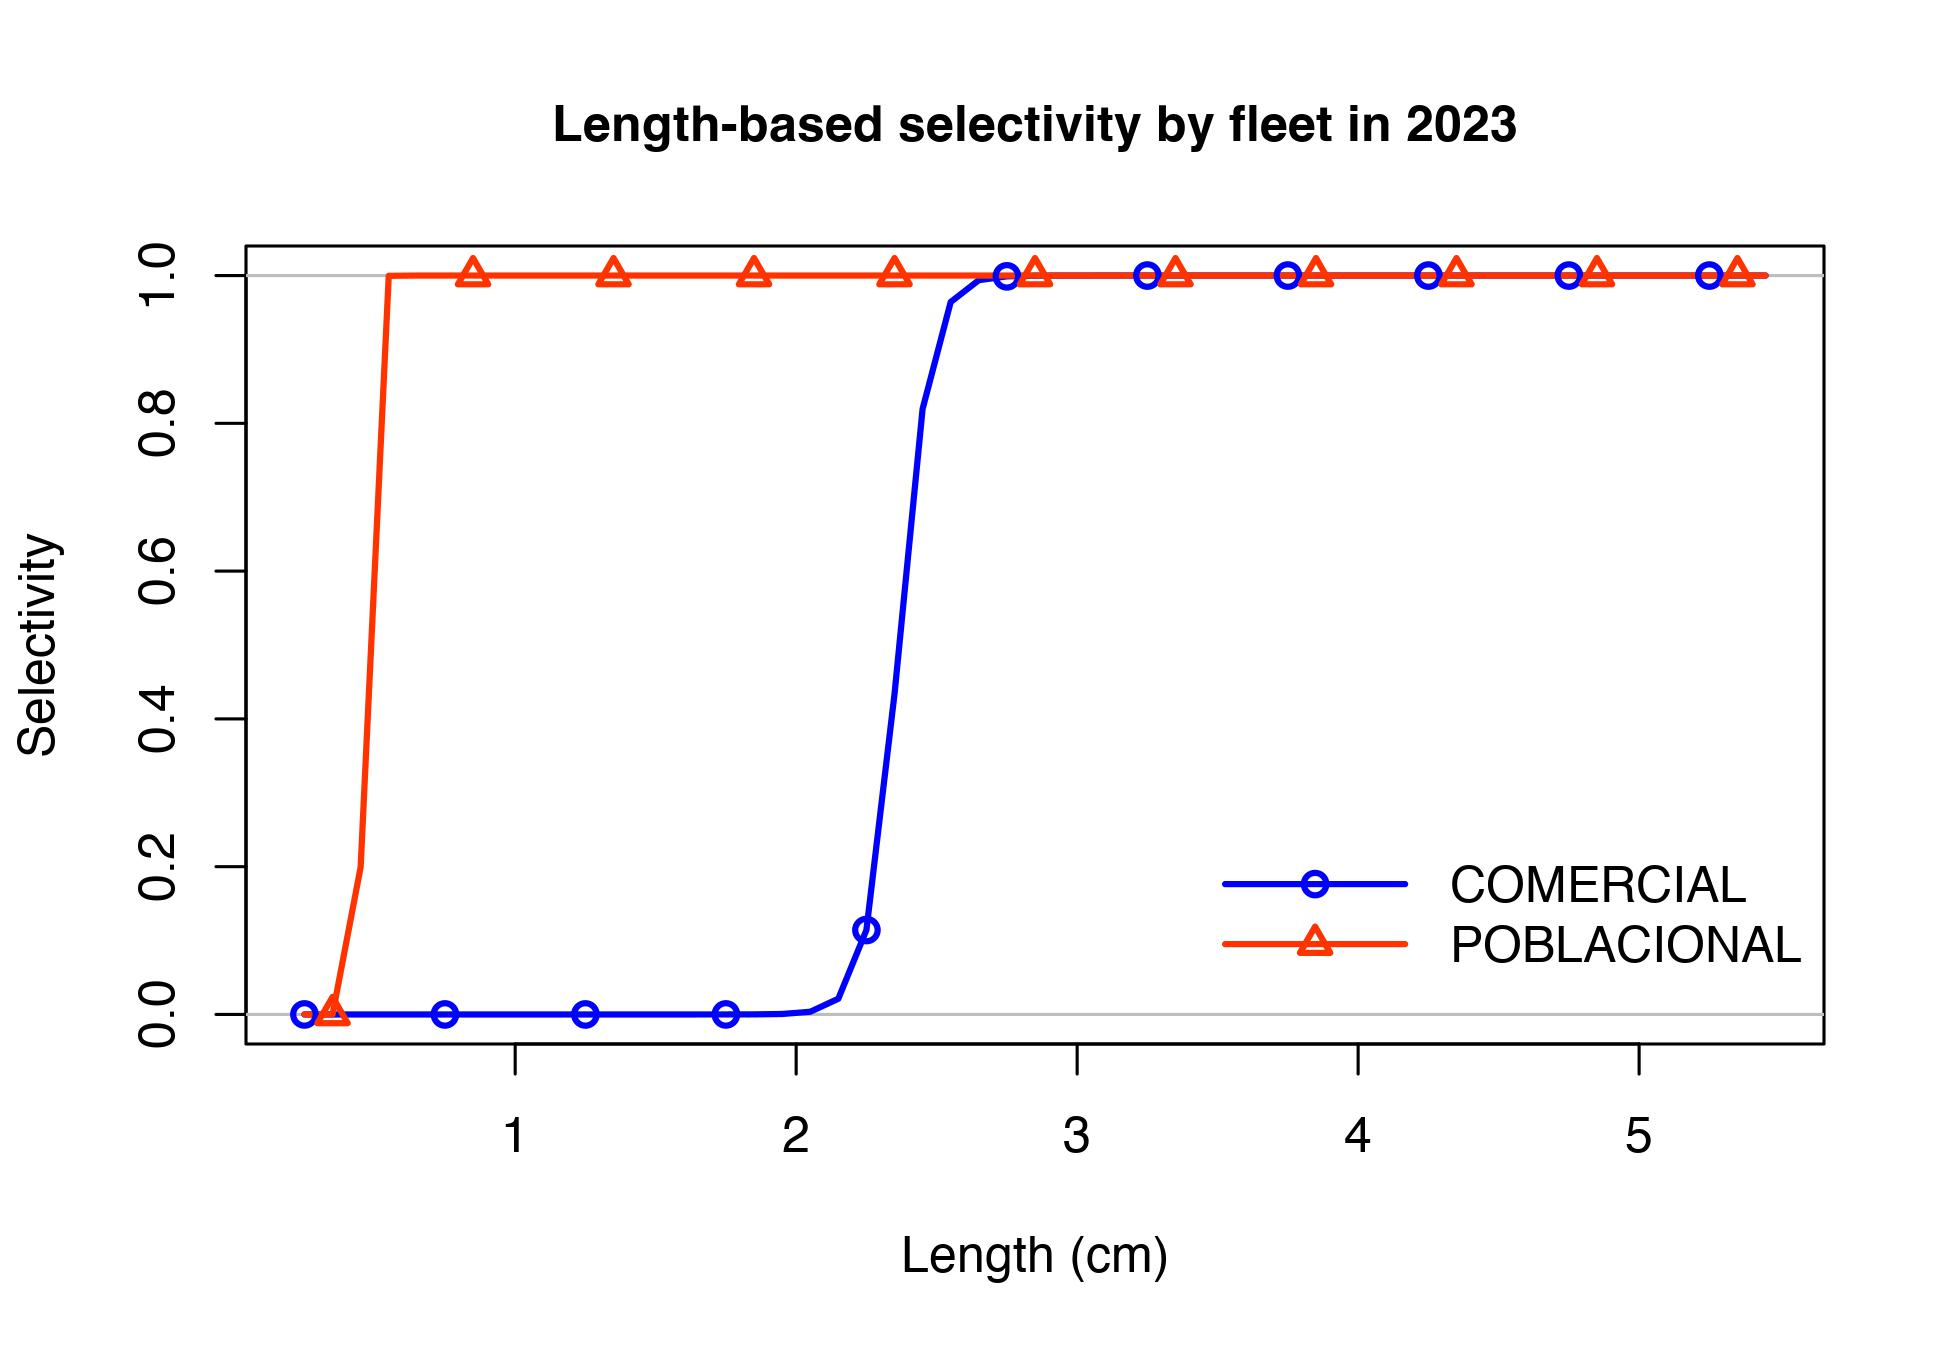
\includegraphics[width=0.8\linewidth]{Dtrunculus_SS3_2024_files/figure-latex/sel-1} 

}

\caption{\label{fig:sel}selectivity at length in end year for all fleets shown together para coquina}\label{fig:sel}
\end{figure}

\hypertarget{modelos-alternativos-escenarios}{%
\subsection{2.5. Modelos alternativos (Escenarios)}\label{modelos-alternativos-escenarios}}

Para avanzar en la implementación metodológica, y considerando las fuentes de incertidumbre asociadas a la modelación de stock de coquina, se establecen una serie de modelos alternativo. Estos escenarios dicen relación con el subreporte de este tipo de pesquerias (Galicia paper ref) en particular, con la coquina (ref). Esto dado los niveles de furtivismo que no son reflejados en las cifras oficiales. Por ello, este ejercicio contempló una corrección al alza de los desembarques oficiales provistos por la Junta a traves de IDEASPA. Esto tiene como objetivo identificar el impacto del subreporte en la estimación de variables poblacionales, así como en el status del recurso. Estos escenarios estan descritos en la Tabla \ref{Tab2}.

\begin{table}[h!]
\centering\centering
\caption{\label{tab:unnamed-chunk-9}\label{Tab2}Descripción de los escenarios alternativos al modelo base inicial (S1).}
\centering
\fontsize{10}{12}\selectfont
\begin{tabular}[t]{ll}
\toprule
Escenarios & Descripción\\
\midrule
\cellcolor{gray!10}{S01} & \cellcolor{gray!10}{Solo Desembarque e Índice}\\
S1 & Flota comercial y poblacional, Desembarque, Índice, Composiciones de Tallas\\
\cellcolor{gray!10}{S2} & \cellcolor{gray!10}{S1 + Vector Desembarques desde 1990 asumido en 250 por año}\\
S3 & S1 + Vector desembarques ponderado por 1.5\\
\cellcolor{gray!10}{S4} & \cellcolor{gray!10}{S1 + Vector desembarques ponderado por 2}\\
\addlinespace
S5 & S1 + Vector desembarques ponderado por 2.5\\
\bottomrule
\end{tabular}
\end{table}

\pagebreak

\hypertarget{resultados-modelo-base-s1}{%
\section{\texorpdfstring{3. RESULTADOS (Modelo Base \texttt{s1})}{3. RESULTADOS (Modelo Base s1)}}\label{resultados-modelo-base-s1}}

\hypertarget{ajustes-y-residuos}{%
\subsection{3.1 Ajustes y residuos}\label{ajustes-y-residuos}}

En relación a los análisis de bondad de ajuste más clásicos, los ajustes a las tallas muestran un adecuado desempeño, siguiento las modas anuales de la estructura de tallas poblacional (Figura \ref{fig:fitpob}) y comercial (Figura \ref{fig:fitcom}).

\begin{figure}[H]

{\centering \includegraphics[width=0.8\linewidth]{s1/plots/comp_lenfit_flt2mkt0} 

}

\caption{\label{fig:fitpob}Fits Length comps, whole catch, POBLACIONAL para coquina}\label{fig:fitpob}
\end{figure}

\begin{figure}[H]

{\centering \includegraphics[width=0.8\linewidth]{s1/plots/comp_lenfit_flt1mkt0} 

}

\caption{\label{fig:fitcom}Fits Length comps, whole catch, COMERCIAL para coquina}\label{fig:fitcom}
\end{figure}

A su vez, el modelo captura la tendencia de tallas medias tallas poblacional (Figura \ref{fig:lenfit}) y comercial (Figura \ref{fig:lenfit2}).

\pagebreak

\hypertarget{variables-poblacionales}{%
\subsection{3.2. Variables poblacionales}\label{variables-poblacionales}}

\begin{table}[ht!]
\centering\centering
\caption{\label{tab:unnamed-chunk-11}\label{Tab4}Series de tiempo estimados por el modelo inicial (S1). Reclutamiento (millones de ind.),  biomasa desovante (en toneladas), Captura (t) y mortalidad por pesca (año-1).}
\centering
\fontsize{9}{11}\selectfont
\begin{tabular}[t]{ccccc}
\toprule
Año & Reclutamientos & \makecell[c]{Biomasa\\desovante} & Captura & \makecell[c]{Mortalidad\\por pesca}\\
\midrule
\cellcolor{gray!10}{2004} & \cellcolor{gray!10}{62296.6} & \cellcolor{gray!10}{131.49} & \cellcolor{gray!10}{23.00} & \cellcolor{gray!10}{0.19}\\
2005 & 61230.7 & 129.68 & 50.00 & 0.48\\
\cellcolor{gray!10}{2006} & \cellcolor{gray!10}{59486.4} & \cellcolor{gray!10}{116.10} & \cellcolor{gray!10}{38.00} & \cellcolor{gray!10}{0.41}\\
2007 & 56959.7 & 97.43 & 56.01 & 0.68\\
\cellcolor{gray!10}{2008} & \cellcolor{gray!10}{53952.3} & \cellcolor{gray!10}{91.39} & \cellcolor{gray!10}{70.11} & \cellcolor{gray!10}{1.09}\\
\addlinespace
2009 & 49618.8 & 75.70 & 73.90 & 1.58\\
\cellcolor{gray!10}{2010} & \cellcolor{gray!10}{46620.0} & \cellcolor{gray!10}{57.28} & \cellcolor{gray!10}{80.40} & \cellcolor{gray!10}{2.65}\\
2011 & 46487.8 & 41.16 & 30.01 & 0.84\\
\cellcolor{gray!10}{2012} & \cellcolor{gray!10}{47197.6} & \cellcolor{gray!10}{33.12} & \cellcolor{gray!10}{85.27} & \cellcolor{gray!10}{2.95}\\
2013 & 54359.4 & 41.84 & 74.82 & 3.95\\
\addlinespace
\cellcolor{gray!10}{2014} & \cellcolor{gray!10}{31108.3} & \cellcolor{gray!10}{26.72} & \cellcolor{gray!10}{80.63} & \cellcolor{gray!10}{4.00}\\
2015 & 38914.1 & 27.11 & 48.49 & 3.94\\
\cellcolor{gray!10}{2016} & \cellcolor{gray!10}{58124.2} & \cellcolor{gray!10}{17.08} & \cellcolor{gray!10}{34.99} & \cellcolor{gray!10}{1.57}\\
2017 & 52284.3 & 21.79 & 86.55 & 3.03\\
\cellcolor{gray!10}{2018} & \cellcolor{gray!10}{119431.0} & \cellcolor{gray!10}{37.18} & \cellcolor{gray!10}{72.14} & \cellcolor{gray!10}{2.85}\\
\addlinespace
2019 & 128653.0 & 31.37 & 176.82 & 4.00\\
\cellcolor{gray!10}{2020} & \cellcolor{gray!10}{111082.0} & \cellcolor{gray!10}{59.33} & \cellcolor{gray!10}{191.15} & \cellcolor{gray!10}{4.00}\\
2021 & 103375.0 & 64.28 & 167.60 & 4.00\\
\cellcolor{gray!10}{2022} & \cellcolor{gray!10}{46126.8} & \cellcolor{gray!10}{56.98} & \cellcolor{gray!10}{135.34} & \cellcolor{gray!10}{2.91}\\
2023 & 60944.1 & 55.60 & 24.72 & 0.58\\
\bottomrule
\end{tabular}
\end{table}

Los componentes de verosimilitud, además de los análisis de residuales permiten identificar entre los bloques de modelos cuales de las configuraciones presenta un desempeño adecuado en términos estadísticos de ajuste a la información. Este modelo es el seleccionado como caso base y sirve para desplegar sus principales salidas para fines informativos de indicadores; como biomasa desovante y pronóstico y biomasa desovante relativa (Figura \ref{fig:ssb}).

\begin{figure}[H]

{\centering 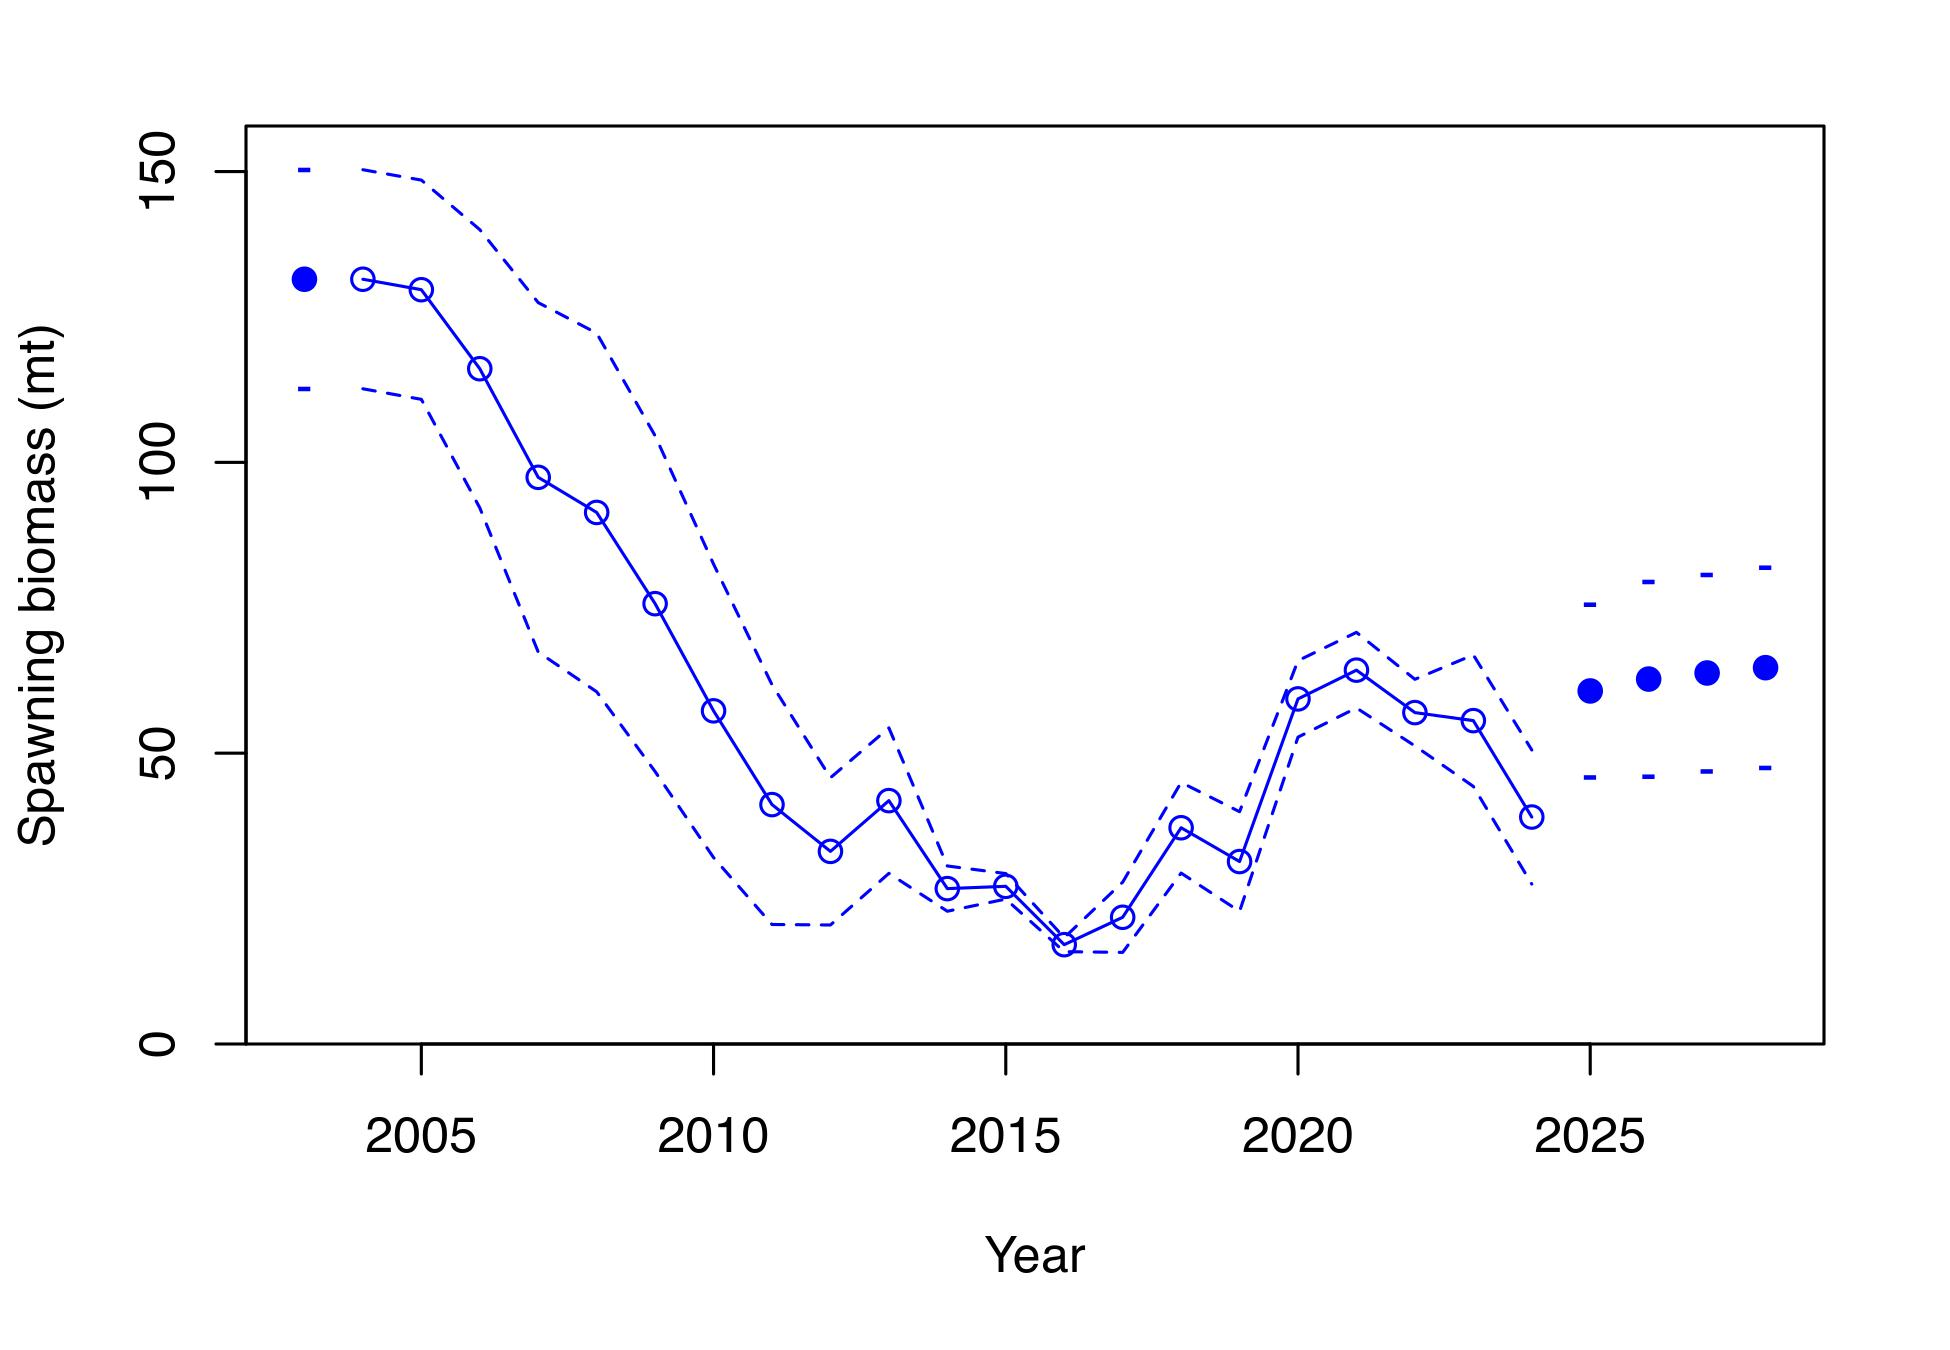
\includegraphics[width=0.8\linewidth]{Dtrunculus_SS3_2024_files/figure-latex/ssb-1} 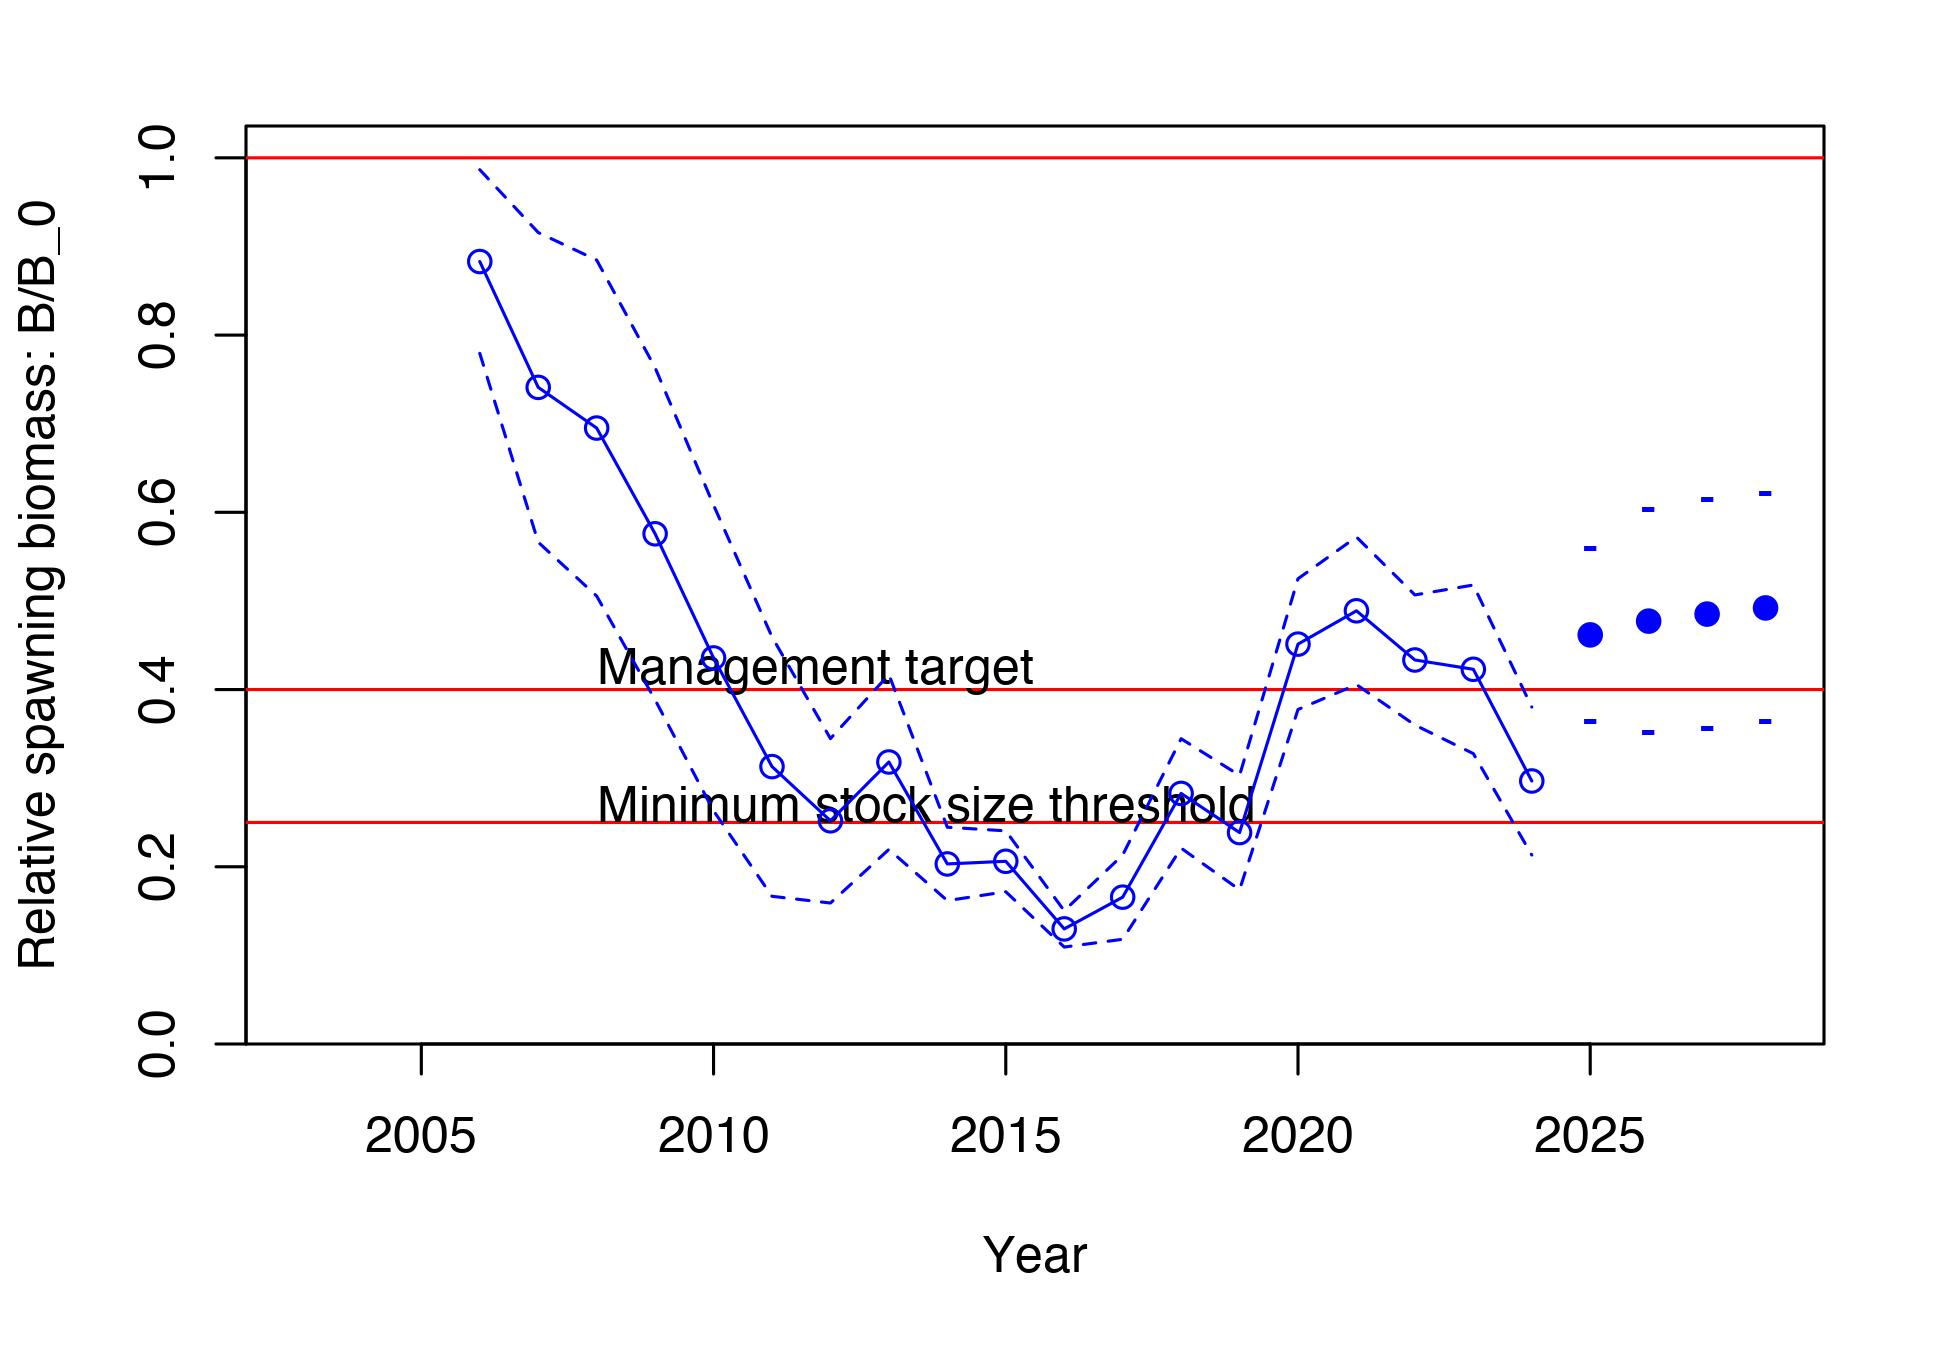
\includegraphics[width=0.8\linewidth]{Dtrunculus_SS3_2024_files/figure-latex/ssb-2} 

}

\caption{\label{fig:ssb}Spawning output with forecast with ~95\% asymptotic intervals and relative spawining biomass to coquina}\label{fig:ssb}
\end{figure}

\hypertarget{anuxe1lisis-retrospectivo}{%
\subsection{3.3. Análisis Retrospectivo}\label{anuxe1lisis-retrospectivo}}

Se siguieron los procedimientos explicados en el objetivo 1 de este reporte, para evaluar la idoneidad
del modelo y dichos procedimientos se han probado en 6 implementaciones (escenarios) diferentes del
modelo inicial (S1).

Dado que la variabilidad del índice rho de Mohn depende de la historia de vida (usualmente
mayor para especies de vida corta) y que el estadístico parece insensible a F, Hurtado-ferro et al. (\protect\hyperlink{ref-Hurtado2014}{2015})
propusieron que el patrón retrospectivo de alguna de las variables biológico-pesqueras indicadas es
preocupante si los valores del índice Mohn's rho son superiores a 0,20 o inferiores a -0,15 para especies
de vida larga, o superiores a 0,30 o inferiores a -0,22 para especies de vida corta. Esto es un factor relevante al momento de hacer diagnosis con recursos como la coquina. Los resultados de el análisis de sesgo para cada escenario son represetados por el parámetro de Rho en la Figura \ref{fig:retro}.

\begin{figure}[H]

{\centering 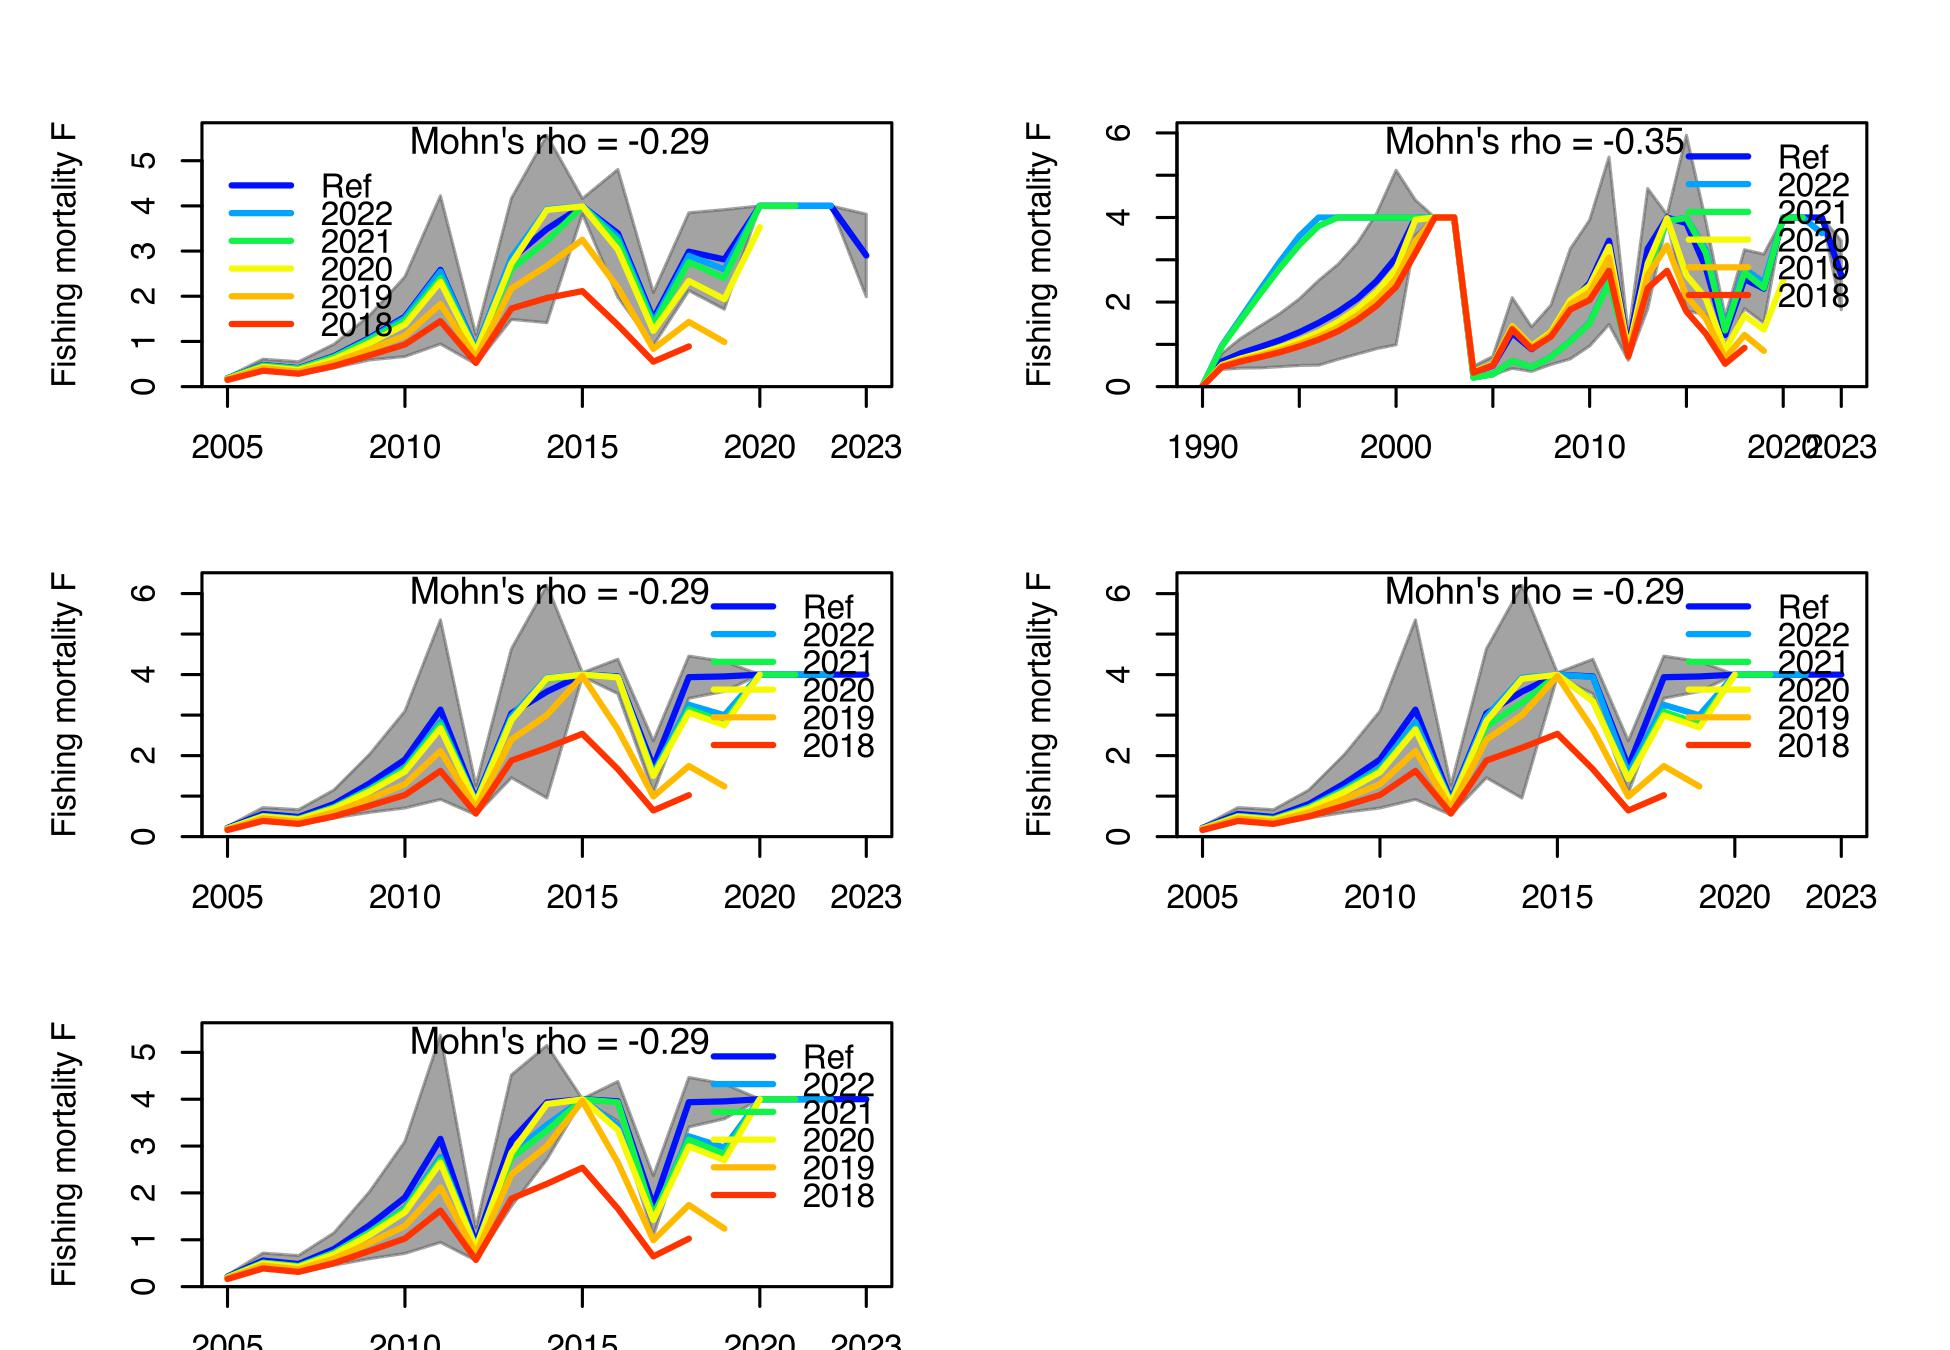
\includegraphics{Dtrunculus_SS3_2024_files/figure-latex/retro -1} 

}

\caption{\label{fig:retro}Patrón restrospectivo para cada esnario modelado en coquina}(\#fig:retro )
\end{figure}

\hypertarget{hindcast-cross-validation-and-prediction-skill}{%
\subsection{3.4. Hindcast Cross-Validation and prediction skill}\label{hindcast-cross-validation-and-prediction-skill}}

Implementing the Hindcast Cross-Validation (HCxval) diagnostic in Stock Synthesis requires the same model outputs generated by \texttt{r4ss:SS\_doRetro()}. As a robust measure of prediction skill, we implemented the mean absolute scaled error (MASE). In brief, the MASE score scales the mean absolute. Regarding (A MASE score \textgreater{} 1 indicates that the average model forecasts are worse than a random walk. Conversely, a MASE score of 0.5 indicates that the model forecasts twice as
accurately as a naïve baseline prediction; thus, the model has prediction skill.

\begin{center}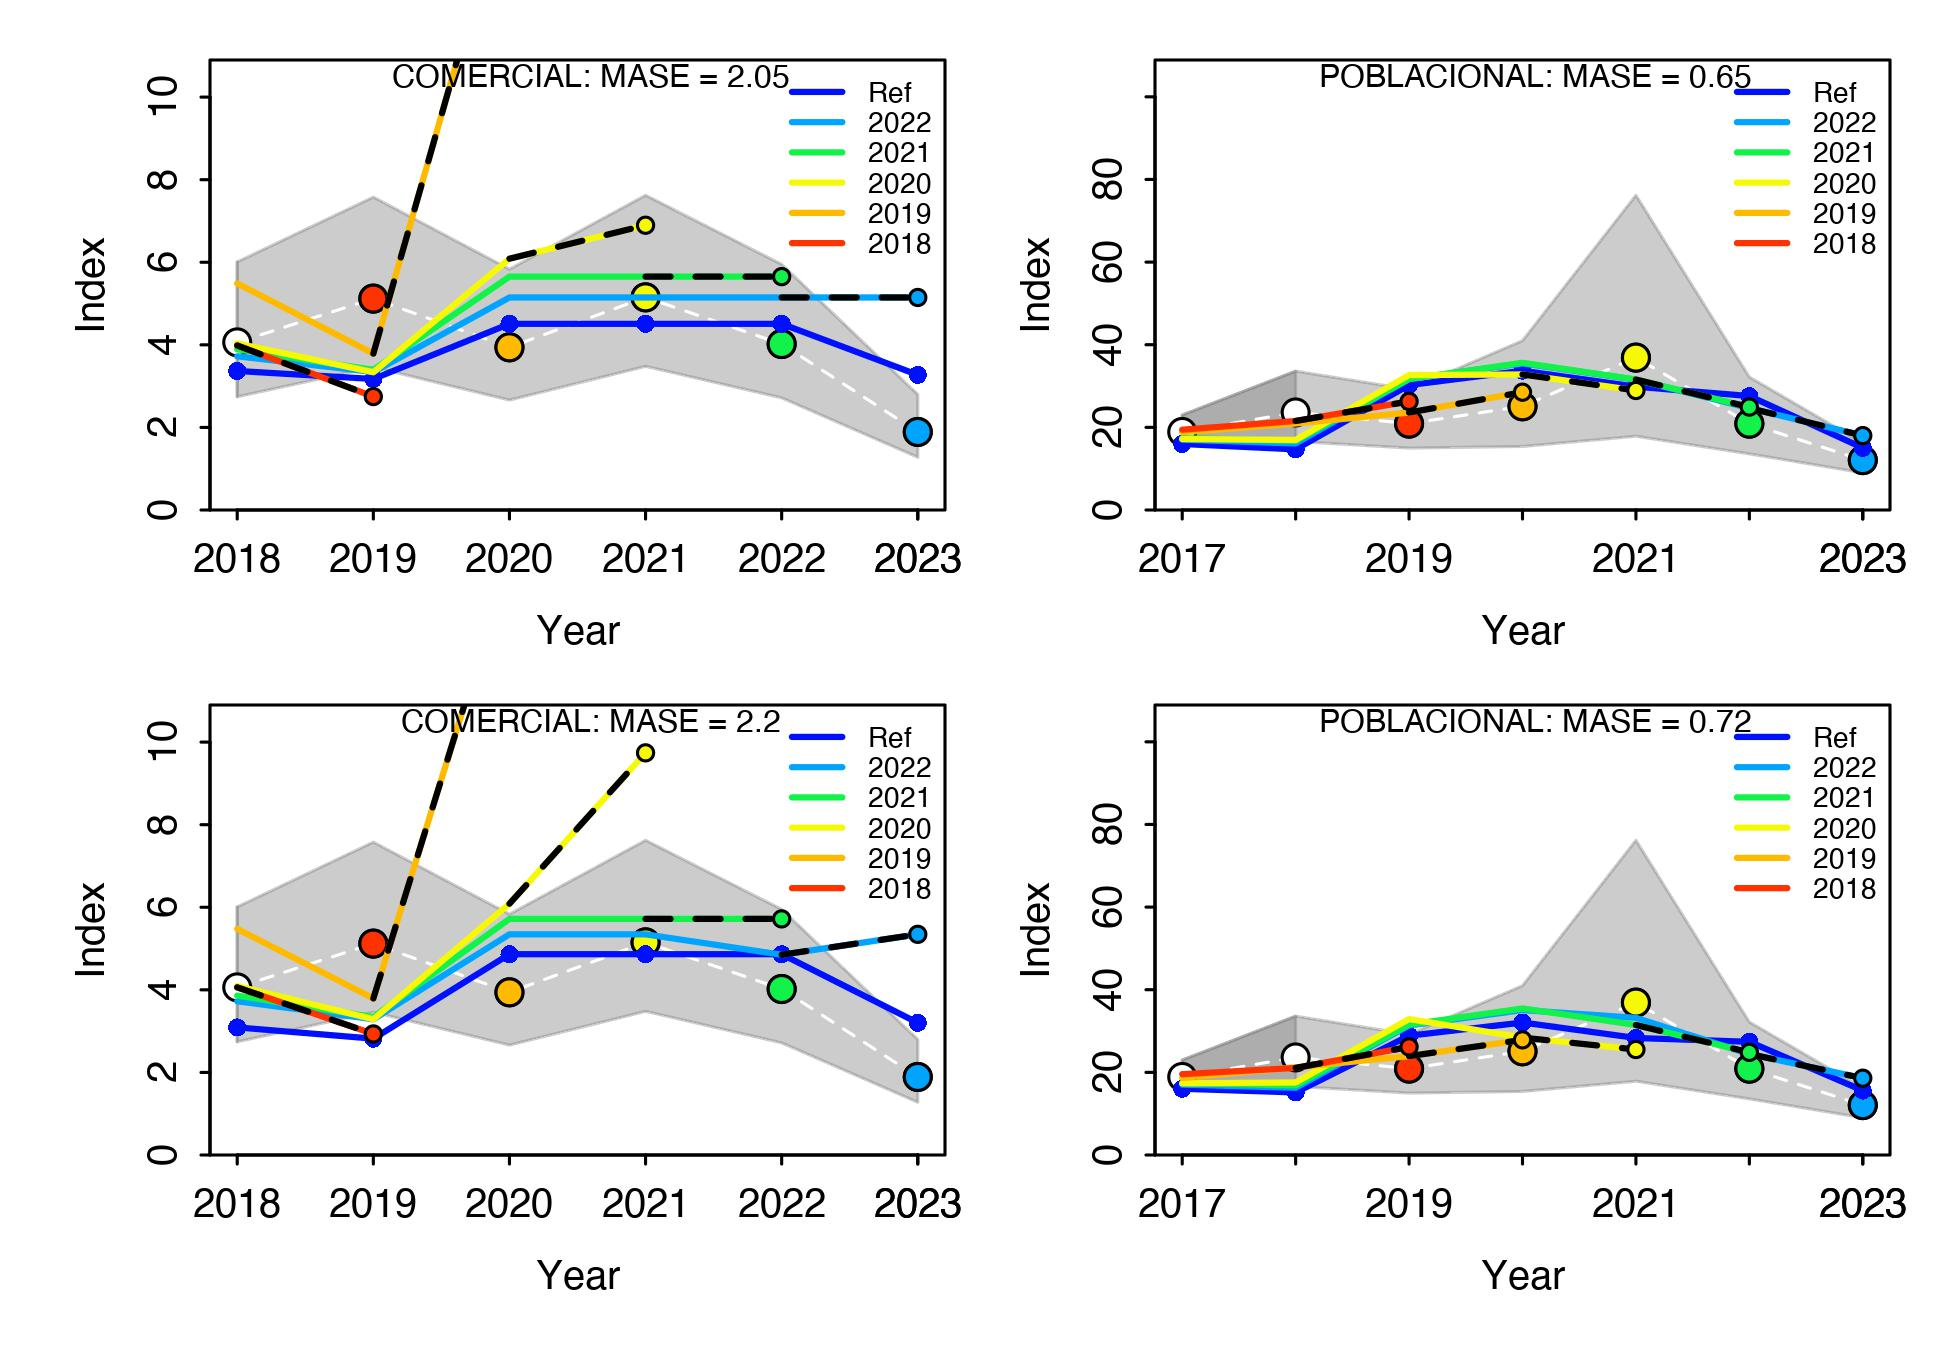
\includegraphics{Dtrunculus_SS3_2024_files/figure-latex/unnamed-chunk-15-1} \end{center}

\begin{center}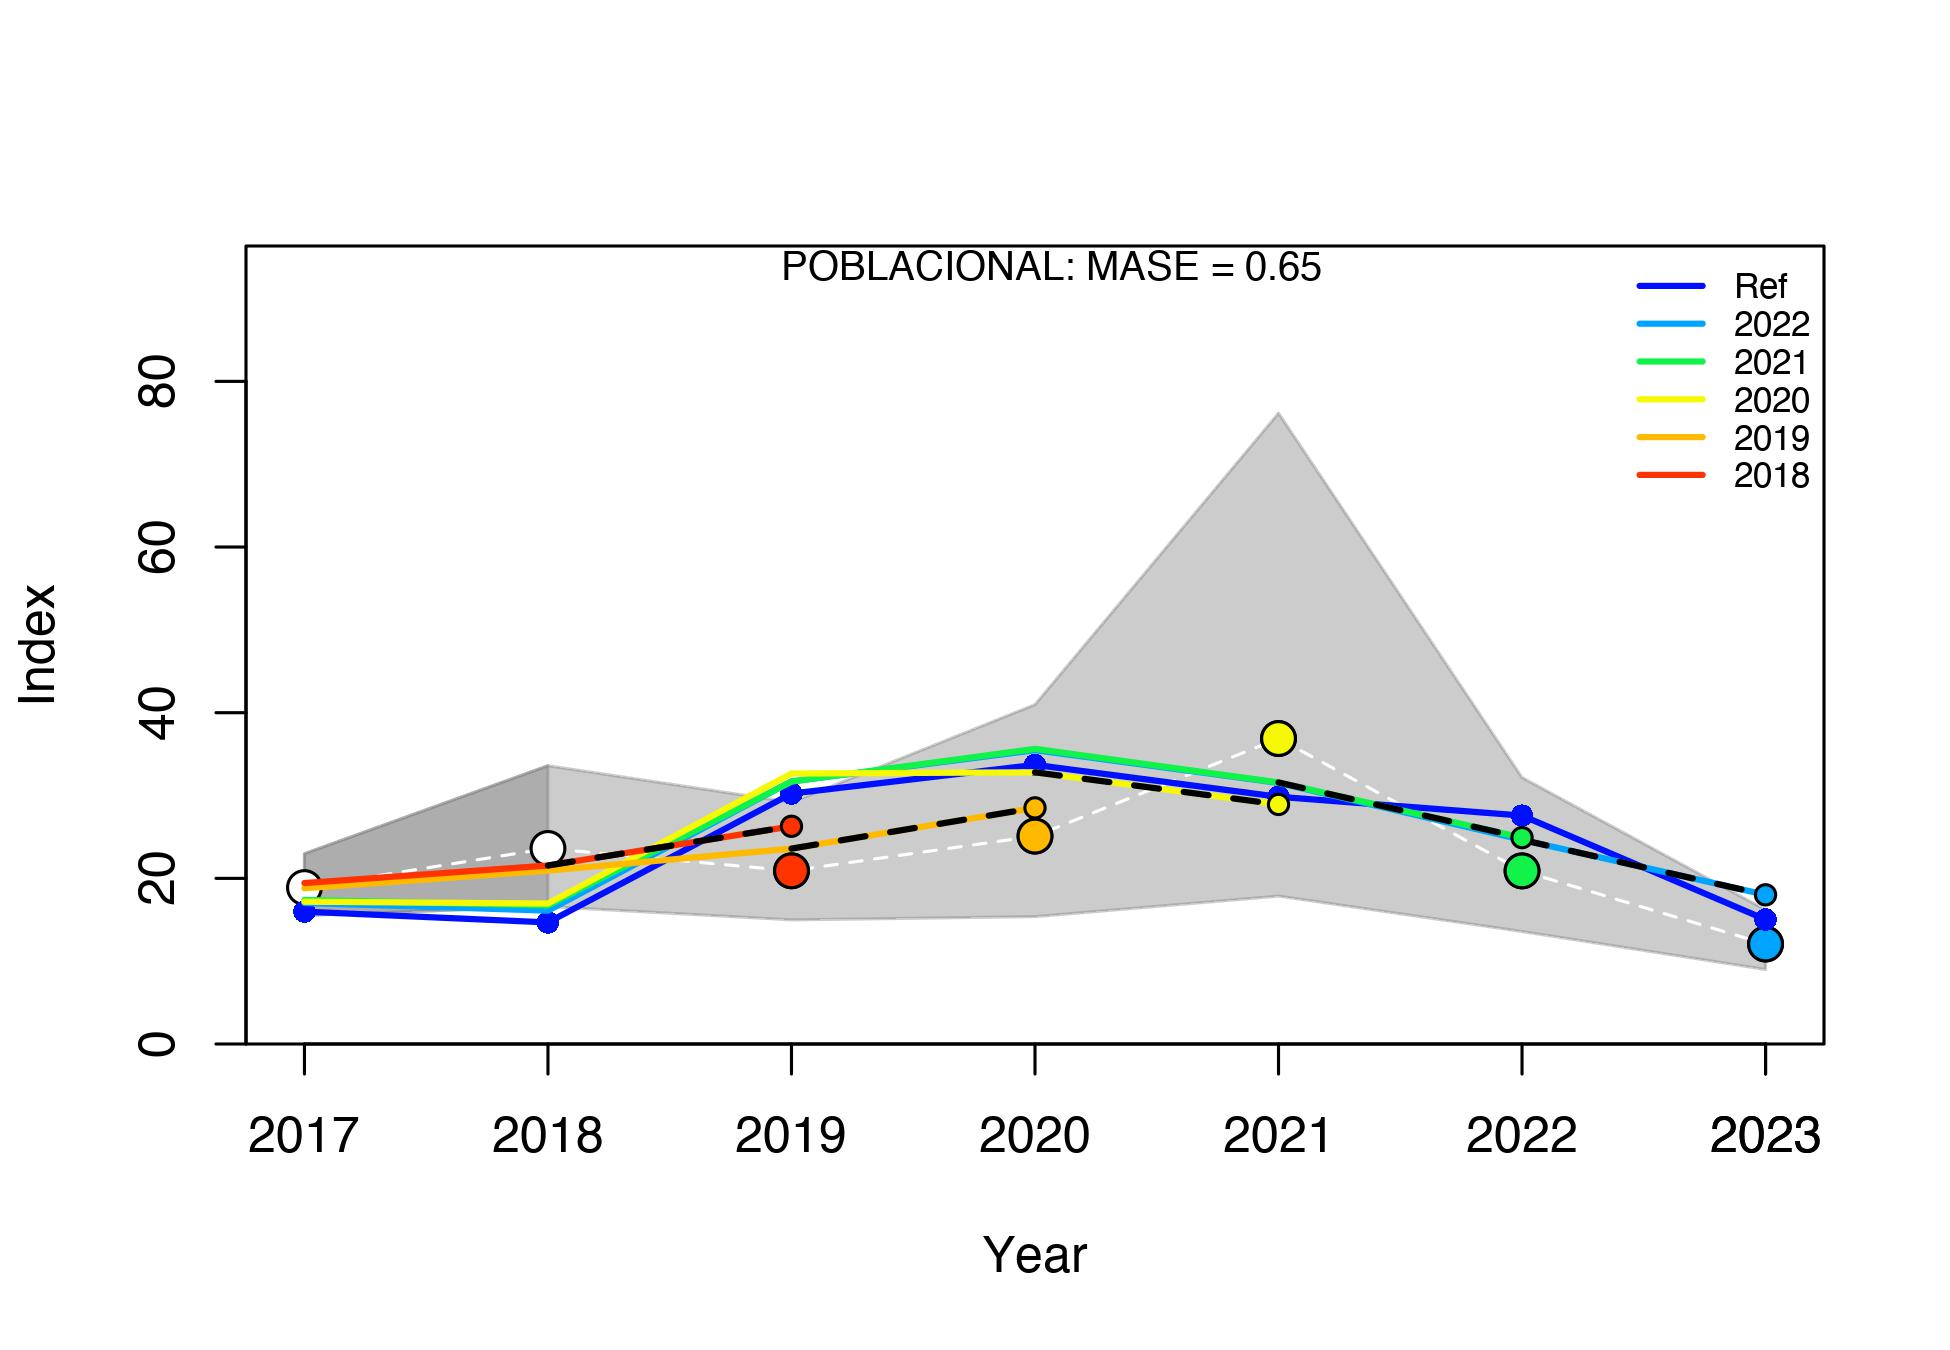
\includegraphics{Dtrunculus_SS3_2024_files/figure-latex/unnamed-chunk-15-2} \end{center}

\begin{table}[H]
\centering
\caption{\label{tab:unnamed-chunk-16}Rho parameter in SSB model s01}
\centering
\begin{tabular}[t]{llrr}
\toprule
type & peel & Rho & ForcastRho\\
\midrule
SSB & 2022 & -0.0053309 & -0.2037735\\
SSB & 2021 & -0.0172189 & -0.0152340\\
SSB & 2020 & 0.1961537 & 0.0138184\\
SSB & 2019 & 1.2906896 & 0.2479760\\
SSB & 2018 & 1.5609331 & 2.5961966\\
\addlinespace
SSB & Combined & 0.6050453 & 0.5277967\\
\bottomrule
\end{tabular}
\end{table}

\begin{table}[H]
\centering
\caption{\label{tab:unnamed-chunk-16}Rho parameter in F model s01}
\centering
\begin{tabular}[t]{llrr}
\toprule
type & peel & Rho & ForcastRho\\
\midrule
F & 2022 & 0.0000000 & 0.3780084\\
F & 2021 & 0.0000000 & 0.0000000\\
F & 2020 & -0.1174900 & 0.0000000\\
F & 2019 & -0.6487907 & 0.0000000\\
F & 2018 & -0.7023415 & -0.7822336\\
\addlinespace
F & Combined & -0.2937244 & -0.0808450\\
\bottomrule
\end{tabular}
\end{table}

\begin{table}[H]
\centering
\caption{\label{tab:unnamed-chunk-16}Rho parameter in SSB model s2}
\centering
\begin{tabular}[t]{llrr}
\toprule
type & peel & Rho & ForcastRho\\
\midrule
SSB & 2022 & 0.0781307 & -0.2318261\\
SSB & 2021 & -0.0194848 & -0.0142870\\
SSB & 2020 & 0.5004057 & 0.1021839\\
SSB & 2019 & 1.2680436 & 0.4409779\\
SSB & 2018 & 1.2052425 & 1.8933489\\
\addlinespace
SSB & Combined & 0.6064675 & 0.4380795\\
\bottomrule
\end{tabular}
\end{table}

\begin{table}[H]
\centering
\caption{\label{tab:unnamed-chunk-16}Rho parameter in F model s2}
\centering
\begin{tabular}[t]{llrr}
\toprule
type & peel & Rho & ForcastRho\\
\midrule
F & 2022 & -0.0925900 & 0.5192489\\
F & 2021 & 0.0000000 & 0.0000000\\
F & 2020 & -0.3751975 & 0.0000000\\
F & 2019 & -0.6348327 & -0.1960775\\
F & 2018 & -0.6391313 & -0.7141121\\
\addlinespace
F & Combined & -0.3483503 & -0.0781881\\
\bottomrule
\end{tabular}
\end{table}

\pagebreak

\hypertarget{comparaciuxf3n-de-resultados-entre-modelos}{%
\subsection{3.5. Comparación de resultados entre modelos}\label{comparaciuxf3n-de-resultados-entre-modelos}}

\begin{verbatim}
##  [1] 3.065958e+02 3.518800e+02 9.995759e-01 1.035935e+00 1.363499e+00
##  [6] 1.488604e+00 4.200000e+00 6.514884e+00 2.799352e+05 3.403843e+05
## [11] 8.855721e-01 1.055893e+00 7.996957e+01 4.439662e+00 1.363499e+00
## [16]           NA           NA
\end{verbatim}

Lo analisis comparados, muestran las estimaciones de cada escenario propuesto para los casos de fraccion de biomasa virginal (Figura \ref{fig:biov}), desvio de los reclutamientos (Figura \ref{fig:devrec}) y mortalidad por pesca (Figura \ref{fig:ftotal}).

\begin{figure}[H]

{\centering \includegraphics[width=0.8\linewidth]{Fig/compare4_Bratio_uncertainty} 

}

\caption{\label{fig:biov}Comparación escenario de razon de Biomasa}\label{fig:biov}
\end{figure}

\begin{figure}[H]

{\centering \includegraphics{Fig/compare12_recdevs_uncertainty} 

}

\caption{\label{fig:devrec}Comparación escenarios de desvios de reclutamiento}\label{fig:debrec}
\end{figure}

\begin{figure}[H]

{\centering \includegraphics[width=0.8\linewidth]{Fig/compare8_Fvalue_uncertainty} 

}

\caption{\label{fig:ftotal}Comparación escenarios de Mortalidad por Pesca}\label{fig:ftotal}
\end{figure}

\hypertarget{status}{%
\section{4. STATUS}\label{status}}

\begin{verbatim}
## 
##  starter.sso with Bratio: SSB/SSB0 and F: _abs_F 
## 
\end{verbatim}

\begin{center}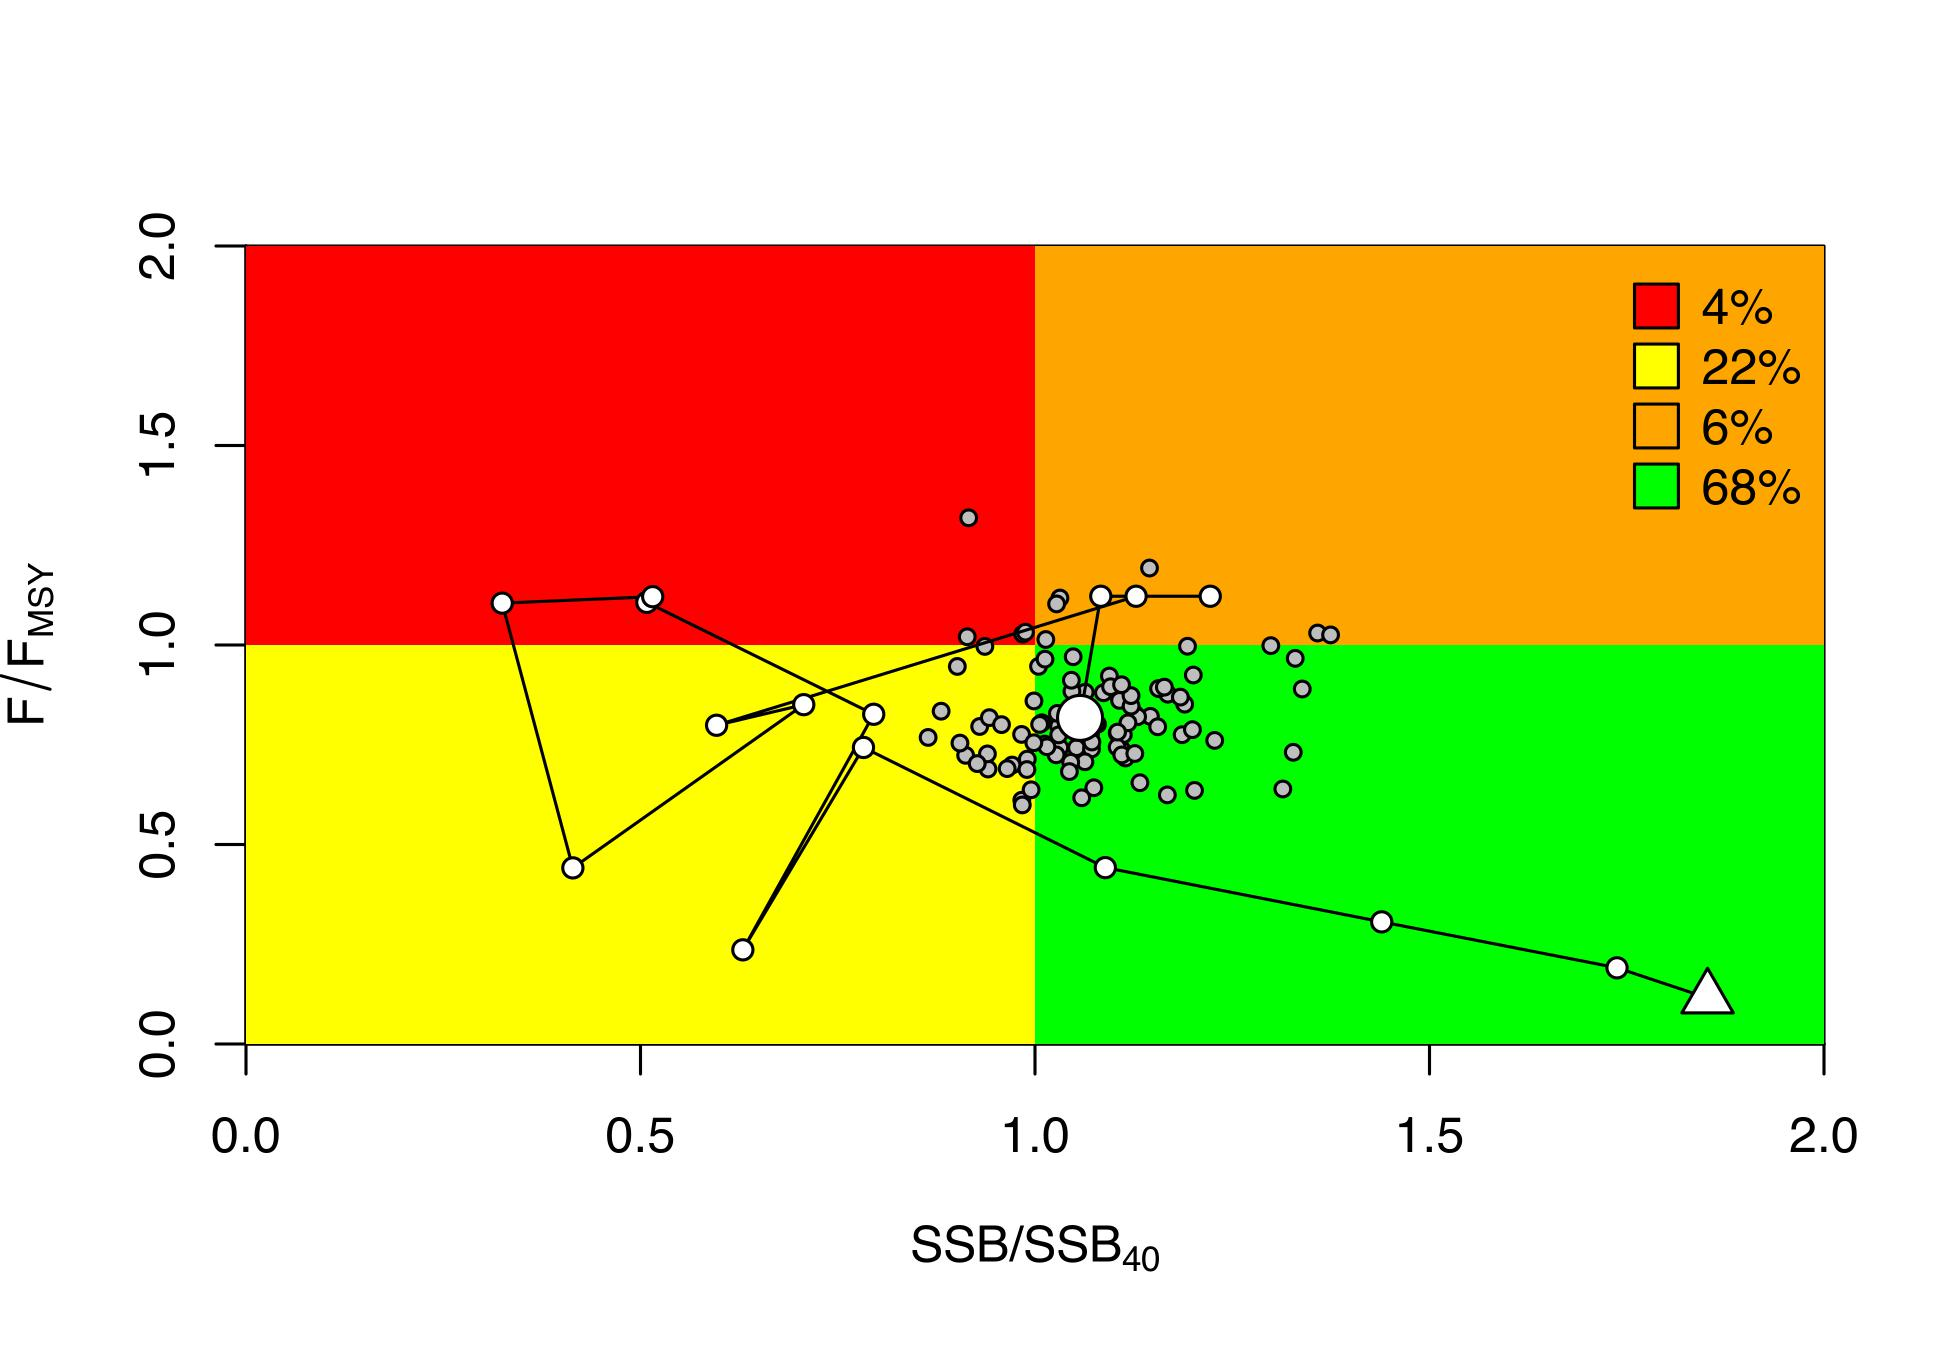
\includegraphics{Dtrunculus_SS3_2024_files/figure-latex/unnamed-chunk-19-1} \end{center}

\begin{verbatim}
## 
##  starter.sso with Bratio: SSB/SSB0 and F: _abs_F 
## 
\end{verbatim}

\begin{center}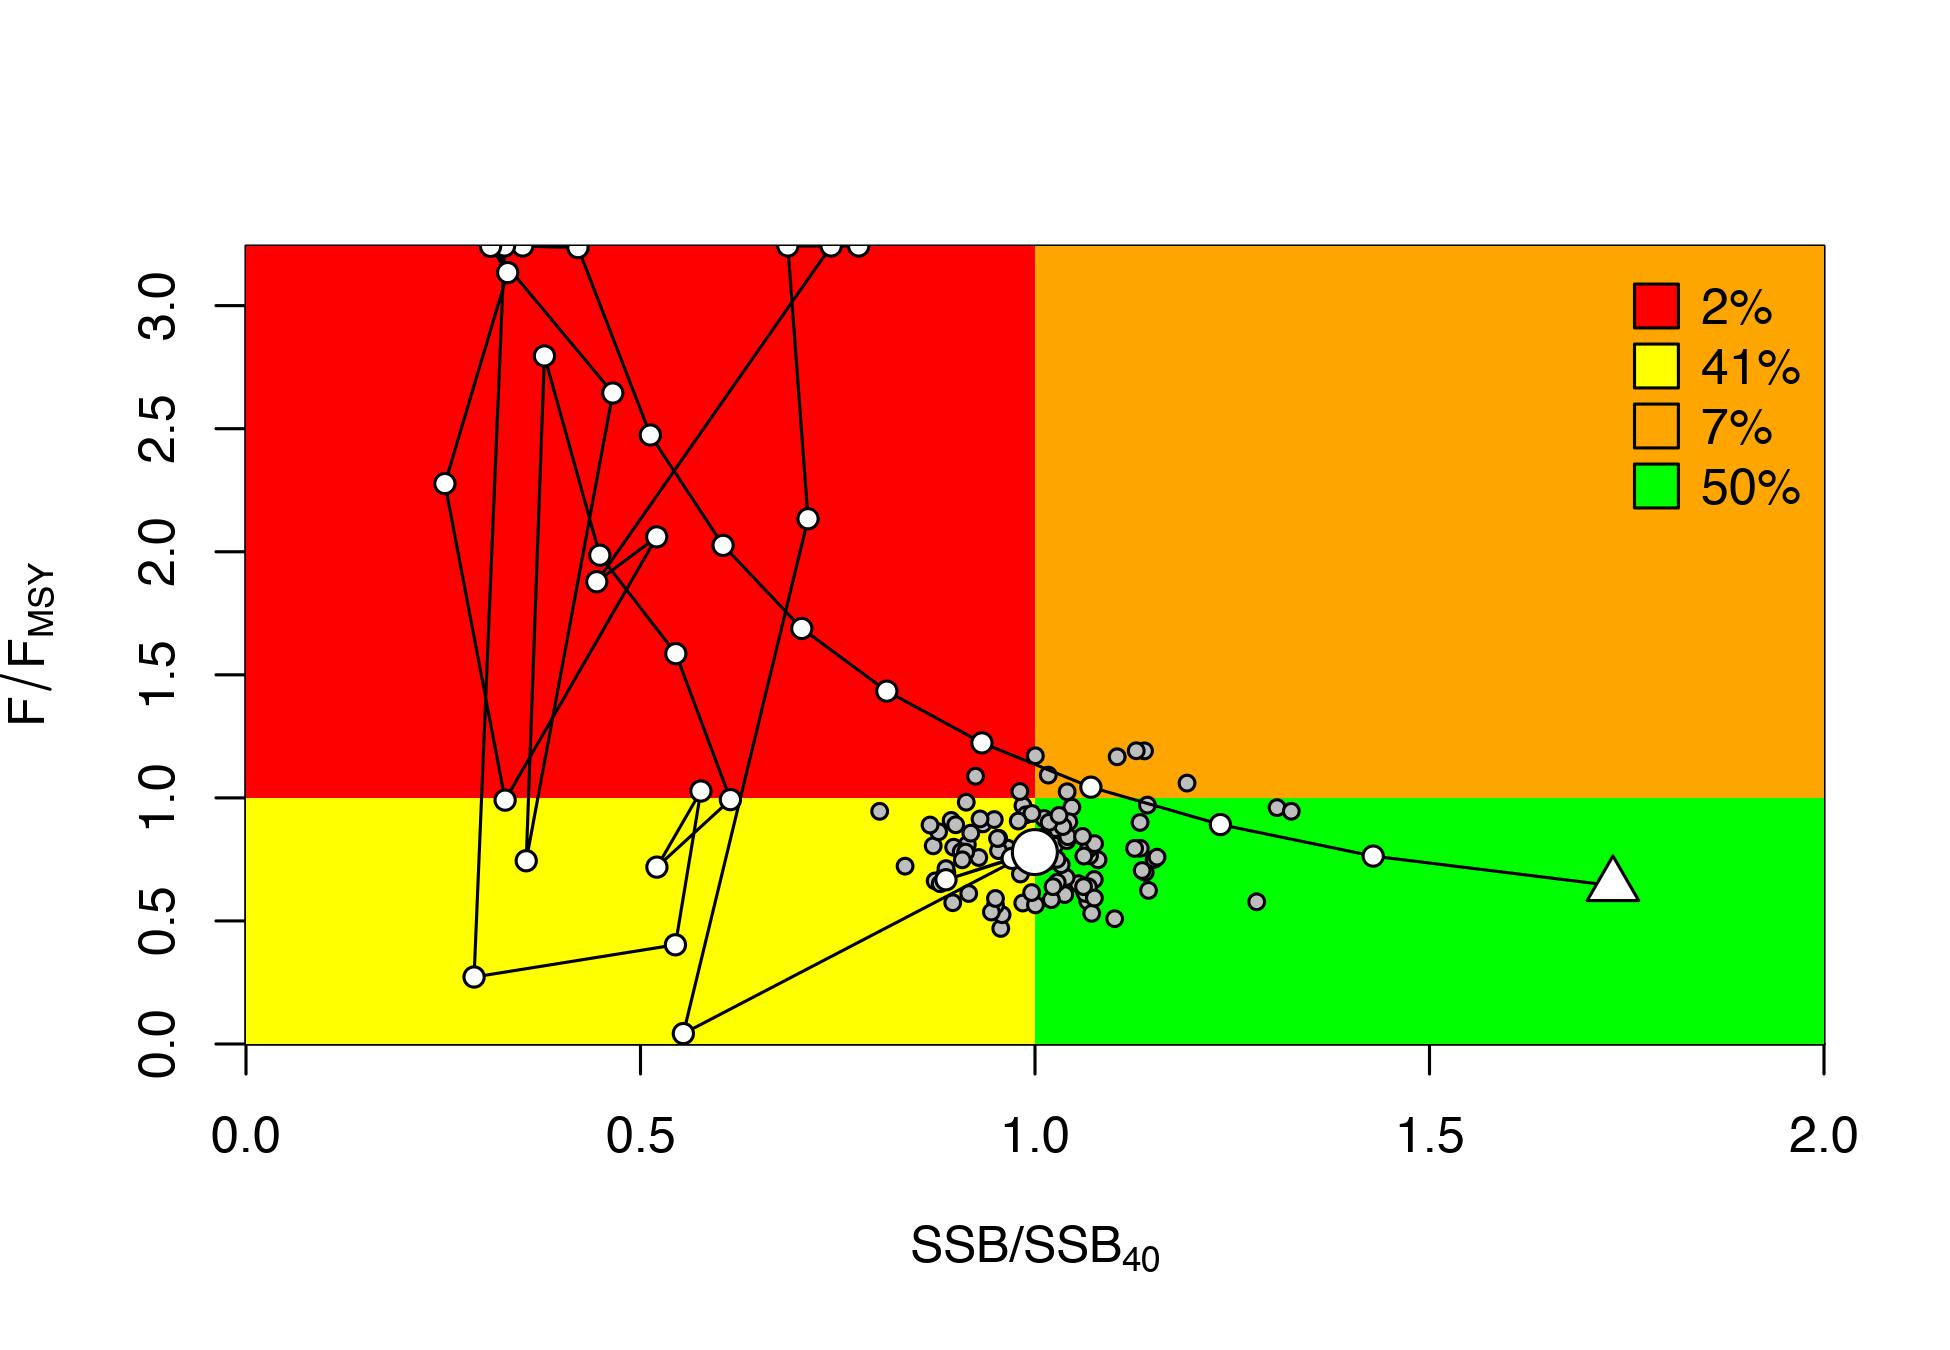
\includegraphics{Dtrunculus_SS3_2024_files/figure-latex/unnamed-chunk-19-2} \end{center}

\pagebreak

\hypertarget{progreso}{%
\section{5. PROGRESO}\label{progreso}}

\begin{itemize}
\item
  explicar PBR
\item
  Definir estatus
\item
  \texttt{S01} falta implementar modelo
\item
  Falta mirar perfiles de verosimilitud
\end{itemize}

\pagebreak

\hypertarget{referencias}{%
\section*{6. REFERENCIAS}\label{referencias}}
\addcontentsline{toc}{section}{6. REFERENCIAS}

\hypertarget{refs}{}
\begin{CSLReferences}{1}{0}
\leavevmode\vadjust pre{\hypertarget{ref-Caddy2004}{}}%
Caddy, J. F. (2004). {Current usage of fisheries indicators and reference points , and their potential application to management of fisheries for marine invertebrates 1}. \emph{Canadian Journal of Fisheries {\&} Aquatic Sciences}, \emph{1324}(December 2002), 1307--1324. \url{https://doi.org/10.1139/F04-132}

\leavevmode\vadjust pre{\hypertarget{ref-Hurtado2014}{}}%
Hurtado-ferro, F., Szuwalski, C. S., Valero, J. L., Anderson, S. C., Cunningham, C. J., Johnson, K. F., Licandeo, R., Mcgilliard, C. R., Monnahan, C. C., Muradian, M. L., Ono, K., Vert-Pre, K. A., Whitten, A. R., \& Punt, A. E. (2015). {Looking in the rear-view mirror: bias and retrospective patterns in integrated, age-structured stock assessment models}. \emph{ICES Journal of Marine Science}, \emph{72}, 99--110.

\leavevmode\vadjust pre{\hypertarget{ref-Methot2013}{}}%
Methot, Richard D., \& Wetzel, C. R. (2013). {Stock synthesis: A biological and statistical framework for fish stock assessment and fishery management}. \emph{Fisheries Research}, \emph{142}, 86--99. \url{https://doi.org/10.1016/j.fishres.2012.10.012}

\leavevmode\vadjust pre{\hypertarget{ref-Methot2023}{}}%
Methot, Richard D., Wetzel, C. R., Taylor, I. G., Doering, K., \& Jhonson, K. (2023). \emph{{Stock Synthesis User Manual Version 3.30.21}}. NOAA Fisheries Seattle, WA.

\leavevmode\vadjust pre{\hypertarget{ref-Taylor2019}{}}%
Taylor, I. (2019). {Using R for Stock Synthesis Installing R and getting R4SS}. \emph{Fisheries Science}, \emph{November}.

\leavevmode\vadjust pre{\hypertarget{ref-Henning2023}{}}%
Winker, H., Carvalho, F., Cardinale, M., \& Kell, L. (2023). \emph{ss3diags: What the package does (one line, title case)}.

\end{CSLReferences}

\end{document}
